\documentclass[preprint,12pt,authoryear]{elsarticle}

\usepackage[T1]{fontenc}
\usepackage{lmodern}
\usepackage{microtype}
\usepackage{amsmath,amssymb,amsthm,mathtools,bm}
\usepackage{booktabs,multirow,array,tabularx,longtable}
\usepackage{algorithm}
\usepackage{algpseudocode}
\usepackage{graphicx}
\usepackage{subcaption}
\usepackage{tikz}
\usepackage{pgfplots}
\usepackage{xcolor}
\usepackage{enumitem}
\usepackage{siunitx}
\usepackage{url}
\usepackage{hyperref}
\usepackage[nameinlink,capitalise,noabbrev]{cleveref}
\usetikzlibrary{arrows.meta,positioning,calc,fit,backgrounds,shapes.geometric,shapes.symbols,decorations.pathreplacing,patterns,matrix,shadows.blur}
\pgfplotsset{compat=1.18}

\definecolor{msblue}{HTML}{2563A6}
\definecolor{msorange}{HTML}{D86B28}
\definecolor{msgreen}{HTML}{368A55}
\definecolor{mspurple}{HTML}{6B58A6}
\definecolor{msgray}{HTML}{667085}
\definecolor{mslight}{HTML}{F4F6F8}
\hypersetup{colorlinks=true,linkcolor=msblue,citecolor=msgreen,urlcolor=mspurple}
\setlength{\emergencystretch}{2em}
\journal{Journal of Systems Architecture}
\makeatletter
\providecommand{\theHALG@line}{\thealgorithm.\arabic{ALG@line}}
\makeatother

\newtheorem{definition}{Definition}
\newtheorem{assumption}{Assumption}
\newtheorem{lemma}{Lemma}
\newtheorem{proposition}{Proposition}
\newtheorem{theorem}{Theorem}
\newtheorem{corollary}{Corollary}
\theoremstyle{remark}
\newtheorem{remark}{Remark}
\newcommand{\M}{\mathcal{M}}
\newcommand{\I}{\mathcal{I}}
\newcommand{\Pset}{\mathcal{P}}
\newcommand{\Cset}{\mathcal{C}}
\newcommand{\Aset}{\mathcal{A}}
\newcommand{\Tset}{\mathcal{T}}
\newcommand{\DAG}{\mathcal{G}}
\newcommand{\Auth}{\mathsf{Auth}}
\newcommand{\View}{\mathsf{View}}
\newcommand{\Meet}{\mathsf{meet}}
\newcommand{\Expired}{\mathsf{Expired}}
\newcommand{\ms}{\textsc{MemScope}}
\newcommand{\placeholder}{\textcolor{msorange}{\textbf{Placeholder / expected trend only; replace with actual experimental results before submission.}}}

\begin{document}

\begin{frontmatter}

\title{MemScope: A Purpose-Bound Memory Service for Mobile Personal Agents}

\author[inst1]{Anonymous Author(s)}
\affiliation[inst1]{organization={Institution withheld for review},city={Anonymous},country={Anonymous}}

\begin{abstract}
Persistent memory lets a mobile personal agent maintain preferences, plans, and safety-relevant facts across sessions, but it also converts transient disclosures into a durable attack surface. Existing Android search primitives authorize at package or schema granularity, while contemporary agent-memory systems optimize what to retain and retrieve. Neither boundary expresses that a memory acquired for one purpose may be consumed only by particular apps and tools, until a specified expiry, nor does it conservatively govern summaries derived from multiple sources. We present \ms, a purpose-bound memory service for mobile personal agents. MemScope places a reference monitor between Android agents and a system-owned persistent store. Every item binds content to provenance, authorized purposes and consumers, app/tool identities, sensitivity, and lifetime; every read carries an authenticated retrieval token derived from the active AppFunction/task context. Authorization precedes semantic ranking, so rejected items do not enter the model context. Derived memories inherit the meet of their cited sources' labels and are admitted only after source and attribution checks. Retrieval-time expiry and background compaction enforce lifetime, while policy-aware eviction separates safety-critical retention from ordinary relevance. Under explicit trust, complete-mediation, and token-authenticity assumptions, we prove admission soundness, monotone restriction of derived labels, returned-plaintext cross-scope non-disclosure, and expiry safety; these properties deliberately do not claim semantic non-inference after an authorized disclosure. We specify an AOSP implementation and a preregistered evaluation on Pixel and Samsung phones using published memory-extraction and poisoning attacks, long-term-memory benchmarks, and multi-app workloads. Because the project contains no completed measurements, all curves and result tables are marked as conceptual or pending rather than presented as empirical evidence.

\end{abstract}

\begin{keyword}
mobile personal agents \sep purpose-bound memory \sep Android \sep persistent memory \sep provenance \sep reference monitor \sep AppSearch \sep label propagation \sep expiry \sep policy-aware eviction
\end{keyword}

\end{frontmatter}

\begin{highlights}
\item MemScope moves persistent personal-agent memory behind an Android reference monitor.
\item Item labels bind provenance, purpose, consumers, app/tool context, sensitivity, and lifetime.
\item Derived summaries conservatively inherit the meet of their cited sources' authorizations.
\item Formal results cover admission soundness and expiry, not unrestricted semantic non-inference.
\item A phone-based protocol separates pending measurements from conceptual expected trends.
\end{highlights}

% Shared MemScope figure grammar. Pure TikZ icons avoid external font dependencies.
\tikzset{
  msbox/.style={draw=msgray, rounded corners=2pt, very thick, fill=white, align=center, minimum height=9mm, text width=27mm, font=\small},
  honest/.style={msbox, draw=msblue, fill=msblue!8},
  defense/.style={msbox, draw=msgreen, fill=msgreen!10},
  adversary/.style={msbox, draw=msorange, fill=msorange!10, dashed},
  theory/.style={msbox, draw=mspurple, fill=mspurple!9},
  infra/.style={msbox, draw=msgray, fill=msgray!8},
  dataflow/.style={-{Stealth[length=2.4mm]}, very thick, draw=msblue, shorten >=2pt, shorten <=2pt},
  controlflow/.style={-{Stealth[length=2.4mm]}, thick, draw=msgray, dashed, shorten >=2pt, shorten <=2pt},
  policyflow/.style={-{Stealth[length=2.4mm]}, very thick, draw=msgreen, shorten >=2pt, shorten <=2pt},
  attackflow/.style={-{Stealth[length=2.4mm]}, very thick, draw=msorange, densely dashed, shorten >=2pt, shorten <=2pt},
  depflow/.style={-{Stealth[length=2.1mm]}, thick, draw=mspurple, shorten >=2pt, shorten <=2pt},
  labelback/.style={fill=white, inner sep=1.3pt, font=\scriptsize},
  group/.style={draw=msgray!65, rounded corners=4pt, dashed, fill=mslight, fill opacity=.45, text opacity=1, inner sep=5pt},
  stage/.style={circle, draw=msblue, fill=msblue, text=white, font=\bfseries\small, minimum size=6mm, inner sep=0pt},
  database/.style={cylinder, shape border rotate=90, aspect=.28, draw=msgray, very thick, fill=msgray!8, align=center, minimum height=12mm, minimum width=21mm, font=\small},
  shield/.style={regular polygon, regular polygon sides=5, shape border rotate=180, draw=msgreen, very thick, fill=msgreen!12, minimum size=11mm},
  phone/.style={draw=msblue, very thick, rounded corners=3pt, fill=msblue!5, minimum width=34mm, minimum height=57mm},
}

\section{Introduction}
\label{sec:introduction}

A useful personal agent must remember. A calendar correction should survive the conversation in which it was made; a recurring accessibility preference should not need to be repeated; a food allergy mentioned weeks earlier may matter to a shopping or restaurant task. Systems such as MemGPT, MemoryBank, and reflective agents show how persistent stores and generated summaries can extend an agent beyond a finite context window \citep{packer2023memgpt,zhong2024memorybank,shinn2023reflexion}. On a phone, however, ``memory'' is not merely a retrieval-quality component. It is a durable, multi-principal data service positioned among applications, tools, system APIs, cloud models, and one person whose disclosures were made in different contexts.

The security mismatch is concrete. Android AppSearch offers a system-wide index and package/schema visibility controls, and AppFunctions exposes typed callable functionality \citep{android2026appsearch,android2026visibility,android2026appfunctions}. These mechanisms identify a caller or function, but they do not natively express that a fact acquired while arranging health care may be used by a medication-reminder tool but not by an advertising or shopping tool; that the authorization expires on a date; or that a summary derived jointly from health and calendar items must retain both restrictions. Conversely, application-level memory libraries normally expose namespaces and retrieval filters chosen by the agent application. A compromised prompt, an over-sharing model, or a malicious tool therefore operates on the same side of the boundary as the data it is supposed to protect.

Recent evidence makes this boundary timely. MEXTRA demonstrates black-box extraction from agent memories \citep{wang2025mextra}; MINJA injects records through ordinary interaction \citep{dong2025minja}; ADAM adapts extraction queries to the apparent memory distribution \citep{lyu2026adam}; and SPORE persists reactivation payloads and uses a malicious tool channel to export records despite user-level isolation \citep{gao2026spore}. ToolPrivacyBench separately shows why task success is not a privacy metric: a tool-using trajectory can complete correctly while sending unnecessary private atoms to intermediate tools \citep{hu2026toolprivacy}. Memory contamination is durable as well: conversational poisoning and multi-record composition can steer later behavior \citep{wang2026hijacking,gao2026mempoison,xie2026memevobench}. These works do not imply that every memory deployment is exploitable in the same way, but they invalidate the assumption that a user namespace is a sufficient authorization boundary.

\subsection{A purpose-bound service boundary}

This paper develops \ms, an Android service that mediates persistent personal-agent memory outside the model. A memory document carries a label containing its provenance, allowed purposes, allowed app/tool consumers, sensitivity class, creation time, and expiry. An agent never selects an arbitrary purpose string and never queries the backing store directly. Instead, a system component issues a signed retrieval token from the active task and AppFunction execution context. The retrieval monitor first constructs an authorized view and only then invokes lexical or vector ranking. Thus an out-of-scope item is not merely down-ranked or hidden by an instruction; its plaintext is absent from the candidate set visible to the ranker and response model.

Derived memories create the less familiar systems problem. An LLM may compress ten messages into a summary, infer a stable preference, or write a reflection used by later tasks. If a new item combines sources, assigning it the least restrictive source label would launder information across contexts. MemScope instead computes the meet of source authorizations: set-valued permissions are intersected, sensitivity is joined upward, and expiry becomes no later than the earliest source expiry. The service requires cited source identifiers and verifies structural attribution before accepting a caller-proposed derivation. A semantic checker may reject unsupported content, but it is not trusted to widen policy. When attribution is uncertain, admission fails closed or the derived item receives a quarantine label.

Lifetime and resource pressure are also authorization concerns. Deleting an index entry in a later maintenance pass is insufficient if an expired item remains readable between expiry and compaction. MemScope checks a trusted monotonic time on every retrieval and performs background deletion as space reclamation rather than as the primary enforcement mechanism. Under storage pressure, policy-aware eviction preserves pinned safety-critical facts when policy permits, while never extending their lifetime or consumer scope. This differs from treating an LLM context cache as the durable record: recent work shows that safety-critical facts can disappear when compression is evaluated without the future question \citep{zhu2026allergy}.

\subsection{Scope and claims}

The formal claims are intentionally narrower than ``memory privacy.'' Given an uncompromised OS service, authentic tokens, complete mediation, correct principal binding, and cryptographic compartment assumptions stated in \cref{sec:threat}, we show that any plaintext item returned by the MemScope API satisfies the declared authorization predicate. We show that a derived label cannot authorize a purpose, consumer, app, tool, or time beyond all its sources. We show that an item whose lifetime has elapsed is not returned, even before physical compaction. These are safety properties of the service interface. They do not prevent an authorized consumer from memorizing or re-transmitting data, do not hide access patterns, and do not provide semantic non-inference over a sequence of individually authorized responses. DP-MemView addresses that complementary cumulative-inference problem under a different interface contract \citep{kim2026dpmemview,dwork2014algorithmic}.

No completed MemScope implementation or measurement dataset was present in the source project. Accordingly, this manuscript does not claim an achieved extraction rate, latency, energy cost, accuracy, or statistical improvement. It contributes a reproducible system design, formal core, prototype plan, and experimental protocol. Conceptual plots make hypotheses inspectable but are visibly labeled as non-results.

\subsection{Contributions}

The work makes five contributions directly expanding the source concept:

\begin{enumerate}[leftmargin=*]
  \item \textbf{Labeled mobile-agent memory.} We define a persistent document abstraction whose enforceable dimensions are provenance, purpose, app/tool consumer, sensitivity, and lifetime, coupled to a retrieval-token protocol rooted in Android task and AppFunction context.
  \item \textbf{Conservative derivation.} We specify source-cited writes, meet-based label propagation, attribution validation, and fail-closed quarantine for summaries and reflections. This prevents the policy widening that would otherwise accompany LLM-based compression.
  \item \textbf{Lifecycle enforcement under mobile constraints.} We separate retrieval-time expiry from physical deletion and introduce a policy-aware eviction objective that preserves utility and designated safety value without changing authorization.
  \item \textbf{A precise security argument.} Under stated assumptions, we prove admission soundness, derived-label monotonicity, interface-level cross-scope non-disclosure, expiry safety, and explicit complexity bounds. We also state counterexamples outside those assumptions.
  \item \textbf{An on-device evaluation protocol.} We define matched experiments on AOSP phones against unscoped memory, identity namespaces, AppSearch visibility, prompt-only instructions, and GAAP-style IFC, using memory extraction/poisoning attacks and long-horizon utility workloads. Every presently unmeasured value remains a placeholder.
\end{enumerate}

\subsection{Paper organization}

\Cref{sec:related} positions MemScope against memory systems, attacks, information-flow control, and mobile platforms. \Cref{sec:preliminaries,sec:system,sec:threat,sec:problem} define the objects and adversary. \Cref{sec:method,sec:algorithm} give the architecture and algorithms. \Cref{sec:theory} presents the formal results; \cref{sec:implementation} maps them to AOSP. \Cref{sec:evaluation} specifies the experiments. \Cref{sec:discussion,sec:limitations} discuss deployment and limits before \cref{sec:conclusion} concludes.

\section{Related Work}
\label{sec:related}

\subsection{Long-term memory for language agents}

Agent-memory research primarily asks what representation and retrieval policy best sustain behavior over long histories. MemGPT uses virtual-context management and multiple memory tiers \citep{packer2023memgpt}; MemoryBank maintains evolving long-term conversational memory \citep{zhong2024memorybank}; generative agents combine observation, reflection, and planning memories \citep{park2023generativeagents}; and Reflexion writes verbal feedback for later trials \citep{shinn2023reflexion}. Retrieval-augmented generation established the broader pattern of retrieving external evidence before generation \citep{lewis2020rag}, while ReAct couples model reasoning with tool actions \citep{yao2023react}. These designs motivate persistent and derived memory but generally place authorization outside the memory abstraction.

LoCoMo and LongMemEval make multi-session recall, temporal reasoning, updates, and abstention measurable \citep{maharana2024locomo,wu2025longmemeval}. Memora emphasizes invalidated facts and forgetting-aware accuracy \citep{uddin2026memora}. These benchmarks are useful for MemScope's utility side, yet authorization requires an additional ground truth: which purpose and consumer may receive each otherwise relevant answer. ProfileFoundry offers structured synthetic people with explicit provenance for constructing such cases without publishing real personal histories \citep{selvam2026profilefoundry}. PersonaChat supplies controlled persona conversations but must be augmented with multi-app and policy metadata \citep{zhang2018personachat}.

Mobile work sharpens the resource problem. A 2026 workshop study compares memory architectures for mobile agents \citep{zhang2026mobilearchitectures}, while MOBIMEM supplies profile, experience, and action memories and reports on-device retrieval behavior \citep{liu2025mobimem}. PA-Bench demonstrates that future-blind compression can discard safety-critical facts \citep{zhu2026allergy}. MemScope is complementary: it does not propose a new semantic memory representation or ranking model. It inserts an authorization and lifecycle boundary before any chosen ranker and constrains derived representations.

\subsection{Closest scope and lifecycle mechanisms}

Audience-Bound Persistent Memory is the closest lifecycle authorization design. It attaches the recording audience to each item, intersects source audiences for derivations, and authorizes context assembly before model use \citep{liu2026audience}. MemScope adopts the same conservative principle but targets a different principal space and enforcement setting: purpose, source, app, tool, consumer, and lifetime in a system-owned mobile store. The comparison must not be overstated; audience authorization is directly overlapping prior work, not a MemScope invention.

MNC binds declassified inter-agent messages to recipient, purpose, forwarding, lifetime, logging, and memory scopes, then uses a non-LLM monitor for downstream enforcement \citep{xu2026mnc}. MemScope specializes this idea to persistent mobile-agent memory: token issuance is connected to Android task/AppFunction context; authorization precedes ranking; labels survive derivation and compaction; and implementation cost is measured on phones. Memory as a Service proposes independently callable and governable memory modules \citep{li2025maas}; MemScope supplies one concrete OS service and policy model rather than a general collaborative-memory agenda.

GAAP tracks private data through agent tools and persistent stores with information-flow control and does not trust the agent to enforce confidentiality \citep{stanley2026gaap}. MemScope shares the external-monitor principle, but its label dimensions, retrieval view, TTL behavior, and eviction policy are tied to durable on-device memory. SSGM proposes governance controls for evolving memory \citep{lam2026ssgm}; Mi-Memory emphasizes provenance, correction, lifecycle artifacts, and edge/cloud deployment \citep{liu2026mimemory}; and MemPrivacy replaces sensitive spans with local placeholders before cloud-side memory processing \citep{chen2026memprivacy}. These are complementary: governance and redaction do not by themselves define per-task authorization over a phone's persistent store.

DP-MemView protects against cumulative attribute inference by controlling response-conditioning views and charging per-attribute privacy ledgers \citep{kim2026dpmemview}. MemScope's deterministic label check does not imply differential privacy and cannot stop inference from multiple authorized disclosures. The systems can be composed: MemScope can first restrict the eligible item set, then a DP interface can mediate aggregate transcript leakage. We therefore cite differential privacy only as a boundary and possible extension, not as the proposed method \citep{dwork2014algorithmic}.

\subsection{Memory attacks and purpose-bound tool disclosure}

MEXTRA extracts private interactions under black-box access \citep{wang2025mextra}; ADAM uses adaptive queries \citep{lyu2026adam}; and SPORE exploits a malicious tool plus persistent reactivation \citep{gao2026spore}. MINJA injects records through query interactions \citep{dong2025minja}. Two MemPoison works expose complementary write-path risks: triggerable conversational poisoning and composition-aware benchmark cases \citep{wang2026hijacking,gao2026mempoison}. MemEvoBench studies longer-horizon drift under adversarial memories and noisy tool outputs \citep{xie2026memevobench}. MemScope's read monitor directly targets cross-scope extraction, while provenance and derived-write admission partly address injection. It does not claim to detect arbitrary false but in-scope facts.

General tool-agent security work supplies broader stress tests. Indirect prompt injection shows that untrusted retrieved content can redirect an integrated application \citep{greshake2023indirect}; AgentDojo offers a dynamic environment for measuring attacks and defenses \citep{debenedetti2024agentdojo}; and ToolEmu uses an emulated sandbox to expose risky tool behavior \citep{ruan2023toolemu}. ToolPrivacyBench is especially relevant because it assigns purpose-specific, need-to-know atoms to tool trajectories \citep{hu2026toolprivacy}. PiSAs similarly applies contextual integrity to multi-user agent outputs, messages, and memory \citep{gupta2026pisas}. MemScope converts these contextual expectations into store admission checks for the single-owner, multi-app mobile case.

\subsection{Information flow, purpose limitation, and expiry}

Security labels have a long formal lineage. Denning models permitted flows with a lattice \citep{denning1976lattice}; decentralized labels attach owner-specific policies and safe relabeling rules \citep{myers1998decentralized,myers2000privacy}; and language-based IFC distinguishes explicit, implicit, and covert flows \citep{sabelfeld2003language}. MemScope uses a small product lattice only for memory authorization. It neither performs whole-program information-flow tracking nor claims noninterference after plaintext crosses the API boundary.

Purpose limitation predates agent memory. Hippocratic databases treat purpose and consent as data-management concerns \citep{agrawal2002hippocratic}, and contextual integrity evaluates whether a flow's actors, attributes, and transmission principles fit a social context \citep{nissenbaum2010privacy}. Riverbed attaches user policy to data processed by distributed services and isolates compatible policies into universes \citep{wang2019riverbed}. MemScope narrows these ideas to task-scoped retrieval and derived-memory propagation, using OS identities that are available on a phone.

Expiry has both logical and physical meanings. Vanish investigated cryptographic self-destruction after a chosen time \citep{geambasu2009vanish}. MemScope does not inherit Vanish's stronger claim that all external copies become unreadable. Its guarantee is that the trusted service returns no expired plaintext; encrypted compartment deletion is defense in depth for stored copies.

\subsection{Android enforcement points}

Android AppSearch offers local and platform storage, ranking, and explicit sharing; PlatformStorage is hosted in the system service, while schema visibility can name authorized packages \citep{android2026appsearch,android2026visibility}. AppFunctions supplies typed function metadata that can ground tool identity and declared task context \citep{android2026appfunctions}. Hardware-backed Keystore/StrongBox can protect compartment keys from ordinary application access \citep{android2026strongbox}. MemScope extends rather than replaces these mechanisms: per-document purpose/lifetime labels and retrieval tokens are more fine grained than current schema/package visibility.

Prior Android research illustrates both dynamic and static flow tracking. TaintDroid joins multiple runtime tracking granularities across smartphone components \citep{enck2010taintdroid}; FlowDroid statically models Android lifecycle and callback behavior \citep{arzt2014flowdroid}. MemScope avoids continuous taint tracking inside the model. It enforces complete mediation at a deliberately small store interface, following classic least-privilege and complete-mediation principles \citep{saltzer1975protection}.

\subsection{Positioning summary}

\begin{table*}[t]
\centering
\caption{Verified closest-work boundary. A check mark records an explicit mechanism, not an overall quality judgment.}
\label{tab:related-comparison}
\small
\resizebox{\textwidth}{!}{%
\begin{tabular}{lcccccc}
\toprule
System & Persistent store & Purpose & App/tool identity & Derived-label meet & Retrieval-time TTL & Phone implementation \\
\midrule
Audience-Bound Memory \citep{liu2026audience} & \checkmark & -- & -- & \checkmark & lifecycle & -- \\
MNC \citep{xu2026mnc} & scoped use & \checkmark & recipient/tool scope & message lineage & \checkmark & -- \\
GAAP \citep{stanley2026gaap} & \checkmark & permissions & \checkmark & IFC labels & policy dependent & -- \\
MemPrivacy \citep{chen2026memprivacy} & \checkmark & -- & edge/cloud boundary & -- & -- & edge component \\
Mi-Memory \citep{liu2026mimemory} & \checkmark & governance & deployment artifacts & provenance & correction/forgetting & edge variant \\
\ms{} (this design) & \checkmark & \checkmark & \checkmark & \checkmark & \checkmark & planned AOSP \\
\bottomrule
\end{tabular}
}
\end{table*}

The novelty claim is therefore bounded: MemScope is a proposed Android enforcement point that combines multi-dimensional per-item scope, authenticated task tokens, derived-item meet propagation, retrieval-time expiry, and mobile resource policies. It is not the first scoped memory proposal, the first information-flow monitor, or the first system to propagate a restrictive label.

\section{Preliminaries and notation}
\label{sec:preliminaries}

\subsection{Principals, purposes, and time}

Let $\Aset$ be the finite set of application identities, each bound to a package name and signing certificate; $\Tset$ the set of tool or AppFunction identities; $\Pset$ a finite purpose vocabulary; and $\Cset$ a set of logical consumers such as an assistant profile or system surface. A task context is
\begin{equation}
q=(a_q,t_q,c_q,p_q,\tau_q,n_q),
\label{eq:query-context}
\end{equation}
where $a_q\in\Aset$, $t_q\in\Tset\cup\{\bot\}$, $c_q\in\Cset$, $p_q\in\Pset$, $\tau_q\in\mathbb{T}$ is trusted monotonic time, and $n_q$ is a fresh nonce. The context is carried inside a system-issued token $\kappa_q=\mathsf{Sign}_{K_{\mathrm{iss}}}(q,e_q)$ with token expiry $e_q$.

Purpose is not inferred from the query string at retrieval time. It is selected from application-authored AppFunction metadata, OS task state, and an optional user-visible purpose confirmation. A classifier may recommend a purpose, but cannot mint a token or expand an item label.

\subsection{Memory items and labels}

\begin{definition}[Labeled memory item]
A memory item is
\begin{equation}
m_i=(i,x_i,z_i,\ell_i,h_i),\qquad
\ell_i=(P_i,A_i,T_i,C_i,s_i,b_i,e_i),
\label{eq:item}
\end{equation}
where $i$ is an immutable identifier, $x_i$ is encrypted content, $z_i$ is provenance, $h_i$ is an integrity digest, $P_i\subseteq\Pset$, $A_i\subseteq\Aset$, $T_i\subseteq\Tset\cup\{\bot\}$, and $C_i\subseteq\Cset$ are authorized sets; $s_i$ is sensitivity in a finite ordered set $\mathbb{S}$; and $b_i,e_i\in\mathbb{T}$ are not-before and expiry times with $b_i<e_i$.
\end{definition}

Provenance $z_i$ records the source package/certificate, source tool or channel, acquisition token identifier, creation time, cited parent identifiers, transformation type, and content digest. Provenance is immutable except for append-only audit annotations.

\begin{definition}[Authorization]
For a verified query context $q$, the item authorization predicate is
\begin{align}
\Auth(m_i,q) \iff {}& p_q\in P_i \wedge a_q\in A_i \wedge t_q\in T_i \wedge c_q\in C_i \notag\\
&\wedge b_i\le \tau_q<e_i \wedge \tau_q<e_q \wedge \mathsf{ValidProv}(z_i).
\label{eq:auth}
\end{align}
\end{definition}

Sensitivity is not an independent read grant. It selects encryption, logging, UI, and retention controls after the set-valued authorization test. A deployment may define clearance constraints, but MemScope never treats a high clearance as permission for an unrelated purpose.

\subsection{Order and meet}

For labels $\ell$ and $\ell'$, write $\ell\preceq\ell'$ when $\ell$ is no more permissive: its allowed sets are subsets, its not-before time is no earlier, its expiry is no later, and its sensitivity is at least as restrictive. For source set $S$,
\begin{equation}
\Meet(S)=\left(
\bigcap_{j\in S}P_j,
\bigcap_{j\in S}A_j,
\bigcap_{j\in S}T_j,
\bigcap_{j\in S}C_j,
\bigvee_{j\in S}s_j,
\max_{j\in S}b_j,
\min_{j\in S}e_j
\right).
\label{eq:meet}
\end{equation}
An empty allowed-set intersection makes the derivation unusable until an explicit, separately authorized relabeling decision occurs. The ordinary derived-write path cannot widen it.

\subsection{Authorized views and ranking}

Given store snapshot $\M_\tau$ and token context $q$, MemScope constructs
\begin{equation}
\View(\M_\tau,q)=\{m_i\in\M_\tau:\Auth(m_i,q)\},
\label{eq:view}
\end{equation}
then evaluates a ranker $R(u_q,\View,k)$ over query text or embedding $u_q$. This order matters: filtering a model-generated top-$k$ list after ranking can leak through scores, identifiers, timing, or explanations and may allow unauthorized candidates to displace authorized ones.

\subsection{Notation table}

\begin{table}[t]
\centering
\caption{Primary notation.}
\label{tab:notation}
\small
\begin{tabularx}{\linewidth}{lX}
\toprule
Symbol & Meaning \\
\midrule
$\M$ & system-owned set of labeled memory items \\
$m_i,x_i,z_i,\ell_i$ & item, encrypted payload, provenance, and label \\
$P_i,A_i,T_i,C_i$ & allowed purposes, apps, tools, and consumers \\
$s_i,b_i,e_i$ & sensitivity, not-before time, and expiry \\
$q,\kappa_q$ & authenticated task context and signed retrieval token \\
$\Auth$ & per-item authorization predicate \\
$\View$ & authorized pre-ranking candidate view \\
$\Meet$ & conservative derived-label meet \\
$\DAG$ & source/derivation directed acyclic graph \\
$B$ & storage budget in bytes \\
$R$ & pluggable lexical/vector/hybrid ranker \\
\bottomrule
\end{tabularx}
\end{table}

\section{System model}
\label{sec:system}

\subsection{Deployment}

MemScope is a privileged Android service in or adjacent to \texttt{system\_server}. The service owns the memory database and exposes a Binder API to enrolled agent applications. The backing index reuses AppSearch query and ranking facilities, but item plaintext, label columns, and compartment keys are not directly accessible to callers. Package identity comes from Binder credentials and signing-certificate verification rather than a caller-provided string. Tool identity comes from the AppFunction invocation chain or a system wrapper for non-AppFunction tools.

\begin{figure*}[t]
\centering
\resizebox{0.98\textwidth}{!}{%
\begin{tikzpicture}[node distance=9mm and 13mm]
  \node[honest, text width=25mm] (user) {\textbf{User / system UI}\\task intent};
  \node[honest, right=of user, text width=28mm] (agent) {\textbf{Personal agent}\\untrusted model};
  \node[adversary, above=8mm of agent, text width=27mm] (tool) {\textbf{Third-party tool}\\AppFunction};
  \node[adversary, below=8mm of agent, text width=27mm] (cloud) {\textbf{Cloud endpoint}\\optional};

  \node[defense, right=18mm of agent, text width=28mm] (issuer) {\textbf{Token issuer}\\app, tool, purpose, TTL};
  \node[defense, right=of issuer, text width=29mm] (monitor) {\textbf{Retrieval monitor}\\verify, filter, audit};
  \node[database, right=15mm of monitor] (store) {\textbf{Scoped store}\\ciphertext + labels};
  \node[defense, above=8mm of store, text width=26mm] (prop) {\textbf{Label propagator}\\meet + attribution};
  \node[infra, below=8mm of store, text width=25mm] (keys) {\textbf{Keystore}\\compartment keys};

  \draw[dataflow] (user.east) -- node[labelback]{request} (agent.west);
  \draw[controlflow] (agent.east) -- node[labelback]{task metadata} (issuer.west);
  \draw[policyflow] (issuer.east) -- node[labelback]{signed token} (monitor.west);
  \draw[dataflow] (monitor.east) to[bend left=24] node[labelback, above=2pt]{query} (store.west);
  \draw[dataflow] (store.west) to[bend left=24] node[labelback, below=2pt]{payload} (monitor.east);
  \draw[dataflow] (monitor.south) -- ++(0,-8mm) -| node[labelback, pos=.28]{ranked view} (agent.south east);
  \draw[attackflow] (tool.south) -- node[labelback]{crafted output} (agent.north);
  \draw[attackflow] (agent.south) -- node[labelback]{possible disclosure} (cloud.north);
  \draw[policyflow] (agent.north east) |- node[labelback, near end]{derived write + source IDs} (prop.west);
  \draw[policyflow] (prop.south) -- node[labelback, right]{restricted label} (store.north);
  \draw[controlflow] (keys.north) -- node[labelback, right]{keys} (store.south);

  \begin{scope}[on background layer]
    \node[group, fit=(issuer)(monitor)(prop)(store)(keys), label={[font=\small\bfseries,text=msgray]above:Android trusted service boundary}] {};
  \end{scope}

  \node[below=16mm of monitor, font=\scriptsize] (ld) {data/model flow};
  \node[right=18mm of ld, font=\scriptsize] (lp) {policy/label flow};
  \node[right=18mm of lp, font=\scriptsize] (la) {adversarial path};
  \draw[dataflow] ([xshift=-12mm]ld.west)--([xshift=-3mm]ld.west);
  \draw[policyflow] ([xshift=-12mm]lp.west)--([xshift=-3mm]lp.west);
  \draw[attackflow] ([xshift=-12mm]la.west)--([xshift=-3mm]la.west);
\end{tikzpicture}
}
\caption{MemScope architecture. The model and tools remain outside the trusted boundary. A task-bound token selects an authorized view before ranking; derived writes use a separate source-cited path. Blue, green, and orange denote ordinary data, trusted enforcement, and adversarially controlled flows, respectively; line style preserves the distinction in grayscale.}
\label{fig:architecture}
\end{figure*}


An agent task begins when a user or system surface invokes an agent with a typed objective. The token issuer maps the task to a purpose in the installed policy, binds the calling app, consumer, and permitted tools, adds a nonce and short expiry, and signs the context. The agent SDK can request memory with this token but cannot change its fields. The retrieval monitor validates the signature and freshness, filters documents by \cref{eq:auth}, calls the chosen ranker on \cref{eq:view}, decrypts only the returned authorized payloads, and records an audit event.

\subsection{Component responsibilities}

\paragraph{Scoped Store.}
The store maintains payload ciphertext, an indexable authorization projection, provenance, integrity digests, derivation edges, TTL metadata, and an append-only audit trail. Label columns are authenticated as associated data. Compartments can group items with compatible sharing and sensitivity policies so that key deletion provides coarse physical erasure.

\paragraph{Retrieval Monitor.}
The monitor is the only plaintext read path. It verifies tokens, constructs authorized views before ranking, enforces result count and query budgets, rate-limits repeated failures, and avoids returning unauthorized identifiers or scores. Audit records refer to opaque item IDs and policy decisions; logging policy prevents the audit stream from becoming a second plaintext store.

\paragraph{Token Issuer.}
The issuer binds purposes to declared functions and user-visible tasks. Tokens are single-task or short-lived, carry a nonce, and enumerate the tools in play. Nested tool calls require attenuation: a child token is no broader than its parent. Token issuance is a policy decision separate from retrieval relevance.

\paragraph{Label Propagator.}
The write path distinguishes direct observations from derivations. Direct items receive defaults from source, task, and data-class policies. Derived items cite existing parent IDs and one or more tokens that share a single composition principal. The propagator checks parent existence and per-parent authorization under that token set, computes \cref{eq:meet}, validates the claimed transformation, and rejects caller-proposed labels broader than the computed meet.

\paragraph{Compactor and eviction controller.}
The controller removes expired ciphertext, rebuilds indexes, rotates compartment keys, and selects eviction candidates under a byte budget. It can prefer retention of authorized safety-critical items, but it cannot extend expiry or grant access. Tombstones and derivation edges prevent a surviving summary from silently losing its lineage.

\subsection{Item lifecycle}

An item moves through \emph{proposed}, \emph{admitted}, \emph{quarantined}, \emph{expired}, \emph{tombstoned}, and \emph{physically compacted} states. Only admitted, unexpired items participate in an authorized view. Quarantined items are unavailable to ordinary retrieval; a local review UI may expose them under a distinct administrative purpose. Logical expiry is instantaneous at the API boundary. Physical deletion is asynchronous and auditable.

\begin{figure*}[t]
\centering
\resizebox{0.98\textwidth}{!}{%
\begin{tikzpicture}[node distance=8mm and 7mm]
  \node[stage] (s1) {1};
  \node[honest, right=2mm of s1, text width=24mm] (intent) {Bind task intent\\and principals};
  \node[stage, right=7mm of intent] (s2) {2};
  \node[defense, right=2mm of s2, text width=24mm] (token) {Issue short-lived\\retrieval token};
  \node[stage, right=7mm of token] (s3) {3};
  \node[defense, right=2mm of s3, text width=24mm] (filter) {Filter labels\\$\Auth(m,q)$};
  \node[stage, right=7mm of filter] (s4) {4};
  \node[honest, right=2mm of s4, text width=23mm] (rank) {Rank authorized\\candidate view};

  \node[stage, below=14mm of s4] (s5) {5};
  \node[honest, left=2mm of s5, text width=23mm] (use) {Use evidence in\\agent/tool call};
  \node[stage, left=7mm of use] (s6) {6};
  \node[theory, left=2mm of s6, text width=25mm] (derive) {Cite sources and\\compute $\Meet(S)$};
  \node[stage, left=7mm of derive] (s7) {7};
  \node[defense, left=2mm of s7, text width=24mm] (verify) {Verify attribution;\\admit or quarantine};
  \node[stage, left=7mm of verify] (s8) {8};
  \node[infra, left=2mm of s8, text width=23mm] (compact) {Expire, audit,\\compact, evict};

  \draw[dataflow] (intent.east)--(s2.west); \draw[policyflow] (token.east)--(s3.west);
  \draw[policyflow] (filter.east)--(s4.west); \draw[dataflow] (rank.south) |- (use.east);
  \draw[dataflow] (use.west)--(s6.east); \draw[depflow] (derive.west)--(s7.east);
  \draw[policyflow] (verify.west)--(s8.east);
  \draw[controlflow] (compact.north west) to[out=160,in=200,looseness=.9] node[labelback, below]{next task} (intent.south west);
\end{tikzpicture}
}
\caption{MemScope read--derive--maintain pipeline. Numbering fixes the security-critical order: authorization occurs before ranking, and derivation checks occur before a generated item becomes retrievable.}
\label{fig:pipeline}
\end{figure*}


\subsection{Policy representation}

Policies are installed manifests signed by the OS, device owner, or enterprise administrator. A rule maps source identities and task metadata to allowed dimensions and lifetime bounds. For example, a calendar availability item may be usable by the scheduling purpose and calendar/messaging tools for 30 days, while a medical item may be restricted to a health purpose and approved health consumer. Rules are combined in a fixed precedence order (mandatory system denial, then enterprise/device-owner, then explicit user rules, then agent defaults), and an access must be permitted at every level. Wildcards are disabled by default: they appear only in signed enterprise/device-owner manifests and are expanded at compile time to the concrete registered set. Purpose identifiers form a closed, versioned taxonomy, and declassification is a separate, object-specific event that does not propagate to descendants. Policy compilation rejects contradictory or unknown-purpose rules and emits a human-readable summary; the frozen v0 semantics appear in \cref{app:policy-frozen}.

\subsection{Consistency and concurrency}

Retrieval operates on a transactionally consistent store snapshot. Token time is checked both before candidate enumeration and before plaintext release. A concurrent expiry, revocation, or label-narrowing event increments a policy epoch; a query whose epoch changed restarts authorization. Derived writes validate all source versions in one transaction. This prevents time-of-check/time-of-use widening without requiring the ranker itself to be trusted.

\section{Threat and privacy model}
\label{sec:threat}

\subsection{Trusted computing base}

We trust the kernel mechanisms that deliver Binder identity, the MemScope service, token-signing code and keys, the policy compiler, the AppSearch-derived storage code that MemScope invokes, trusted monotonic time, and hardware-backed key storage when present. We assume verified boot and ordinary Android sandbox guarantees. These assumptions are substantial and must be tested against the actual prototype; the proof does not survive compromise of this trusted computing base.

The model does not trust the language model, its prompt, an agent application's orchestration logic, retrieved untrusted text, third-party tools, or a cloud memory processor. An agent may be confused, prompt-injected, or intentionally request excessive data. A tool may attempt to export arguments or persist instructions. Other apps may invoke exported surfaces or replay old requests. A stolen database image is considered, but an attacker with an unlocked device plus arbitrary code in the trusted service is out of scope.

\subsection{Adversary classes}

\begin{enumerate}[leftmargin=*]
  \item A \emph{query adversary} interacts with the assistant and adaptively chooses prompts, following the black-box direction of MEXTRA and ADAM \citep{wang2025mextra,lyu2026adam}.
  \item A \emph{write-path adversary} injects content through normal conversations, notifications, or tool outputs, following MINJA and memory-poisoning settings \citep{dong2025minja,wang2026hijacking,gao2026mempoison}.
  \item A \emph{malicious tool} receives calls, returns crafted anchors, and persists reactivation instructions, as in SPORE \citep{gao2026spore}.
  \item An \emph{over-sharing agent} completes a valid task but supplies a tool with more private information than the task requires, as measured by ToolPrivacyBench \citep{hu2026toolprivacy}.
  \item A \emph{storage adversary} obtains an offline copy of the memory database but not an unlocked OS service or hardware-backed compartment key.
\end{enumerate}

\begin{figure*}[t]
\centering
\resizebox{0.98\textwidth}{!}{%
\begin{tikzpicture}[node distance=10mm and 15mm]
  \node[adversary, text width=28mm] (query) {Query attacker\\adaptive probes};
  \node[adversary, below=of query, text width=28mm] (writer) {Poisoning source\\crafted memories};
  \node[adversary, below=of writer, text width=28mm] (badtool) {Malicious tool\\export + persistence};

  \node[honest, right=22mm of writer, text width=31mm] (agent) {Untrusted agent\\prompt and planner};
  \node[shield, right=20mm of agent] (shield) {\small\bfseries MS};
  \node[defense, above=8mm of shield, text width=27mm] (read) {Read monitor\\scope + TTL};
  \node[defense, below=8mm of shield, text width=27mm] (write) {Write monitor\\provenance + meet};
  \node[database, right=20mm of shield] (memory) {Persistent\\memory};

  \node[honest, right=18mm of memory, text width=29mm] (allowed) {Authorized view\\for this task};
  \node[infra, below=of allowed, text width=29mm] (excluded) {Excluded items\\never ranked};

  \draw[attackflow] (query.east) to[bend left=12] (agent.north west);
  \draw[attackflow] (writer.east)--(agent.west);
  \draw[attackflow] (badtool.east) to[bend right=12] (agent.south west);
  \draw[policyflow] (agent.north east) -- (read.west);
  \draw[policyflow] (agent.south east) -- (write.west);
  \draw[policyflow] (read.east) -| (memory.north);
  \draw[policyflow] (write.east) -| (memory.south);
  \draw[dataflow] (memory.east)--(allowed.west);
  \draw[controlflow] (memory.south east) |- node[labelback]{deny / omit} (excluded.west);
  \draw[controlflow] (excluded.north)--(allowed.south) node[midway,right,font=\scriptsize]{disjoint views};
\end{tikzpicture}
}
\caption{Threat-to-control mapping. Read scoping constrains extraction across purposes and tools; provenance and conservative write admission constrain laundering and some poisoning paths. False but in-scope content and inference from authorized answers remain outside the core guarantee.}
\label{fig:threat-map}
\end{figure*}


\subsection{Assets and security goals}

The primary asset is plaintext $x_i$ and its sensitive attributes. Metadata such as item existence, size, access frequency, and timing is a secondary asset but receives only partial protection in this design. The main service goal is:

\begin{quote}
For every successful MemScope read, each returned plaintext item is authorized for the authenticated app, tool, consumer, purpose, and time bound to that read; a derived item is no more permissive than every source used to construct it.
\end{quote}

Supporting goals are token freshness and attenuation, provenance integrity, retrieval-time expiry, audit completeness, fail-closed label propagation, and confidentiality of offline compartment ciphertext under the platform cryptographic assumptions.

\subsection{Explicit non-goals}

MemScope does not guarantee that an authorized response reveals no fact inferable about an unauthorized item. It does not revoke information already copied by an authorized consumer, eliminate model-provider logging after authorized cloud disclosure, hide all access patterns, prevent screen capture, protect against kernel/TEE compromise, or stop false in-scope memories. It does not automatically determine the socially correct purpose policy. It does not claim that hardware-backed encryption causes every cached copy to vanish, unlike the stronger historical objective explored by Vanish \citep{geambasu2009vanish}. Covert channels and timing leakage are measured where feasible but excluded from the core theorem.

\subsection{Complete mediation assumption}

Every durable personal memory read and write by an enrolled agent must traverse MemScope. This is enforceable only if the evaluation disables or instruments alternative vector stores, caches, logs, and direct cloud-memory APIs. If an application maintains a shadow memory, MemScope cannot govern it. The prototype therefore includes an integration audit and a negative-control build with an intentionally bypassing cache to demonstrate the assumption's necessity.

\section{Problem formulation}
\label{sec:problem}

\subsection{Safety and utility objectives}

Let $Q$ be a workload of authenticated task contexts and $G(q)\subseteq\M$ the policy ground-truth items entitled and relevant to task $q$. Let $O(q)$ be the items returned by the store. Authorization violations and misses are
\begin{align}
V(Q)&=\sum_{q\in Q}\sum_{m\in O(q)}\mathbf{1}[\neg\Auth(m,q)],\\
L(Q)&=\sum_{q\in Q}|G(q)\setminus O(q)|.
\end{align}
The safety constraint is $V(Q)=0$ for service-mediated reads under the model. Utility seeks to reduce $L(Q)$, answer error, latency, energy, and storage subject to safety and device budgets.

Because relevance and authorization are different predicates, maximizing conventional recall over all historically relevant items is incorrect. We report \emph{entitled recall}
\begin{equation}
\mathsf{ER@}k=\frac{1}{|Q^{+}|}\sum_{q\in Q^{+}}\frac{|O_k(q)\cap G(q)|}{|G(q)|},
\label{eq:er}
\end{equation}
where $Q^{+}=\{q\in Q: G(q)\ne\emptyset\}$ is the set of queries with nonempty entitled ground truth, alongside out-of-scope retrieval rate. The convention is frozen: queries with $G(q)=\emptyset$ contribute to no denominator and are excluded from the reported mean, a choice that depends only on the method-independent ground truth and not on any method's output, so $\mathsf{ER@}k$ stays comparable across methods evaluated on the identical query set. Reported results also state $|Q^{+}|$ and the number of excluded queries $|Q\setminus Q^{+}|$. A method cannot trade a nonzero violation rate for better entitled recall and still satisfy the principal security property.

\subsection{Derived-item safety}

Let $\DAG=(\I,E)$ be the derivation DAG, where $(j,i)\in E$ means item $i$ cites item $j$ as a source. For parent set $\mathrm{pa}(i)$, a derived item is policy-valid when
\begin{equation}
\ell_i\preceq\Meet(\mathrm{pa}(i))
\quad\wedge\quad
\mathsf{Attributed}(x_i,\{x_j:j\in\mathrm{pa}(i)\}).
\label{eq:derived-validity}
\end{equation}
The first conjunct is deterministic. The second is necessarily approximate for natural-language derivations. MemScope treats a false acceptance by the attribution checker as an integrity risk, not as evidence that a broader label is safe. A deployment can require extractive summaries or user confirmation for high-sensitivity classes.

\subsection{Storage-budget objective}

Let $w_i$ be item size and $y_i\in\{0,1\}$ indicate retention after compaction. For unexpired, policy-retainable items, define estimated future utility $u_i$, safety value $r_i$, sensitivity cost $d_i$, staleness $g_i$, and recomputation cost $c_i$. The planner solves or approximates
\begin{align}
\max_{\bm y}\quad &\sum_i y_i(\alpha u_i+\beta r_i+\gamma c_i-\delta d_i-\eta g_i)\\
\text{s.t.}\quad &\sum_i y_iw_i\le B,\quad y_i=0\text{ if }\tau\ge e_i,
\label{eq:eviction}
\end{align}
with policy-pinned items handled as hard constraints only when their total size fits $B$. If hard constraints exceed the budget, the service raises an explicit resource fault rather than silently discarding safety-critical records. The objective affects retention, never authorization.

\subsection{Design requirements}

The formulation yields seven requirements: (R1) authenticated principal and purpose binding; (R2) per-document enforcement before ranking; (R3) conservative derivation; (R4) retrieval-time expiry; (R5) atomic policy/version checks; (R6) auditable lifecycle transitions; and (R7) bounded mobile overhead. The next sections instantiate these requirements.

\section{MemScope design}
\label{sec:method}

\subsection{Task-rooted retrieval tokens}

The token issuer observes an OS-mediated task start rather than accepting a purpose asserted by the model. Each installed agent declares AppFunctions, human-readable purposes, tool dependencies, and requested memory classes. At task start, the issuer intersects this declaration with device policy, user/enterprise restrictions, and the caller's package identity. The resulting token contains exactly one purpose, one consumer, one caller app, a bounded tool set, a policy epoch, issuance and expiry times, a nonce, and an optional parent-token digest.

Tokens attenuate. If tool $t_1$ calls $t_2$, the child token must satisfy
\begin{equation}
\mathsf{Scope}(\kappa_{t_2})\preceq\mathsf{Scope}(\kappa_{t_1})
\end{equation}
and names $t_2$ as the active consumer. An agent cannot reuse the parent token as a bearer capability at an unrelated tool because Binder caller identity and the invocation-chain digest are verified together. Replay caches reject nonce reuse for one-shot operations; reusable tokens have short TTLs and per-token query budgets.

Purpose taxonomies inevitably contain ambiguity. MemScope therefore separates three cases. A manifest-matched calendar-creation action maps deterministically to a scheduling purpose. A compound task is decomposed into subtasks with separate tokens. An unknown or unusually sensitive mapping requires user confirmation and yields the narrowest applicable token. A language model may help explain the mapping but is not the policy authority. The frozen v0 taxonomy, AppFunction mapping, precedence order, wildcard policy, and declassification rules are specified in \cref{app:policy-frozen}.

\subsection{Pre-ranking authorization}

AppSearch ranking can combine lexical match, schema filters, properties, and application-defined scores \citep{android2026appsearch}. MemScope adds an indexable authorization projection: hashed IDs for allowed apps, tools, consumers, and purposes, plus not-before/expiry ranges and a policy epoch. The store query includes exact/range constraints that form an over-approximation of \cref{eq:auth}. The trusted monitor then rechecks each candidate against the authenticated label before decryption and ranking. This two-stage plan reduces work without trusting the index to make the final decision.

Filtering precedes vector ranking and model reranking. Embeddings can be stored within the same compartment or in a separately protected index. If embeddings are treated as sensitive, unauthorized queries do not receive distances or hit counts. The API pads or coarsens certain errors (no results, invalid scope, rate limit) to reduce trivial enumeration, although complete access-pattern confidentiality is outside the formal guarantee.

\subsection{Direct writes}

A direct write includes payload, source descriptor, active token, requested retention class, and optional user instruction. The service computes policy defaults; the application cannot supply a broader label. Source app and tool are taken from the call chain. Purpose begins at the active task purpose or a policy-defined subset. Consumer sets default to the writing agent and approved system surfaces, never to all installed agents. TTL is capped by the minimum of source policy, task policy, and user choice. High-sensitivity data can require a separate compartment and suppress content-bearing audit fields.

User corrections are versioned rather than overwritten invisibly. A correction creates a new item linked by \texttt{supersedes}; the old item becomes invalid for ordinary retrieval at the commit epoch and is later compacted. This supports Memora-style update evaluation \citep{uddin2026memora} and makes stale-memory reuse observable.

\subsection{Derived writes and attribution}

Summaries, extracted preferences, and reflections use a separate call. The proposal contains generated payload $x_d$, transformation type, ordered parent IDs $S$, one or more active tokens $\Gamma$, and optional spans mapping claims to sources. MemScope performs four checks:

\begin{enumerate}[leftmargin=*]
  \item Every parent exists, is unexpired, and is visible to at least one token in $\Gamma$. All tokens in $\Gamma$ must share one composition principal $(a^*,c^*,p^*)$: the same caller app, consumer, and purpose. Each parent may be reached by a different tool, but only as already authorized for the shared task principal.
  \item Parent versions and digests match the snapshot on which generation occurred.
  \item The proposed label is equal to or more restrictive than $\Meet(S)$.
  \item An attribution verifier finds no material claim unsupported by the cited sources under the configured verifier policy.
\end{enumerate}

The deterministic first three checks establish policy monotonicity. The fourth is a content-integrity heuristic whose errors are measured. For safety-critical or highly sensitive items, the allowed modes can be restricted to extractive selection, structured transforms, or user-confirmed abstraction. An abstractive checker cannot authorize policy widening; a pass merely allows storage under the already conservative meet.

Multi-token composition lets a compound task combine several purpose-compatible views without inventing a super-token. Because the derived label is the meet of every cited parent, adding tokens cannot widen policy; it only decides which parents are eligible to be cited. If the parent intersection is empty, the service does not guess. It may store the item in a quarantined administrative compartment for review, or require separate scoped derivatives. If a parent expires, a derived item already has an expiry no later than that parent and therefore expires too. A direct user grant can create a new declassification event, but that operation is outside ordinary derivation, requires object-specific confirmation, and is recorded as a new provenance edge.

\subsection{Expiry, deletion, and revocation}

Read-time TTL checks are authoritative. The compactor's role is to reclaim space and reduce residual ciphertext, not to decide whether an item is logically accessible. On expiry, the monitor returns neither payload nor content-derived score. The compactor deletes the item, removes index entries, and updates derivation tombstones. If a whole compartment is expired or revoked, destroying its wrapped key accelerates physical erasure.

Revocation differs from expiry because it may occur before $e_i$. Policy epochs make revocation visible to active queries: label narrowing or deletion increments the relevant epoch, and release revalidates it. An audit record contains the rule and version responsible for the decision. Long-running agent tasks must refresh tokens after their expiry; refresh re-evaluates policy rather than extending the old grant automatically.

\subsection{Policy-aware eviction}

When storage exceeds its soft budget, expired and invalidated items leave first. Remaining candidates are grouped by compartment and derivation dependencies. Evicting a parent whose derived item still exists is allowed only if the derivation record retains a digest and audit metadata sufficient for lineage; deployments requiring re-verification pin the parent instead. The objective in \cref{eq:eviction} uses predicted entitled reuse, safety class, sensitivity cost, staleness, and recomputation cost. All learned scores are advisory. Hard policy constraints---for example, retaining a confirmed allergy until a user-specified date---are explicit and size-accounted.

This policy avoids a subtle conflation. Sensitivity can argue for earlier deletion because storage risk is high; safety criticality can argue for retention because forgetting is harmful. MemScope therefore represents both axes rather than treating ``sensitive'' as automatically retained or evicted. If the budget cannot satisfy hard obligations, the UI reports the conflict and requests a storage/policy decision.

\subsection{Auditing and user controls}

The audit log records token ID, caller certificate digest, purpose, tool, opaque item IDs, decision codes, bytes returned, policy version, and timing. Plaintext query and item content are excluded by default. A user-facing view answers: what was remembered, from which source, why it was used, which tool received it, when it expires, and what derived items depend on it. The user can narrow scope, expire an item, correct content, or revoke a tool. Widening requires a distinct confirmation because it changes the information-flow policy.

\subsection{Failure behavior}

MemScope fails closed on invalid signatures, unknown identities, ambiguous tool chains, stale epochs, malformed labels, empty required intersections, unavailable key material, and attribution-checker failures. Fail-closed behavior can reduce utility, so the system distinguishes policy denial from transient infrastructure failure in local diagnostics while presenting a non-revealing error to untrusted callers. The evaluation measures both denied legitimate requests and attempted violations.

\subsection{Why an OS service}

Application libraries cannot reliably mediate competing apps and tool providers, and prompt instructions place enforcement in the component exposed to prompt injection. An OS service already sees package identities, signing certificates, AppFunction metadata, lifecycle events, storage budgets, and hardware-key APIs. AppSearch's package/schema visibility demonstrates a compatible system-service pattern \citep{android2026visibility}; MemScope adds per-document task semantics and derivation lineage rather than discarding the existing index.

\section{Algorithms}
\label{sec:algorithm}

\begin{algorithm}[t]
\caption{MemScope retrieval}
\label{alg:retrieve}
\begin{algorithmic}[1]
\Require signed token $\kappa$, query $u$, result limit $k$
\State $q\gets\mathsf{VerifyToken}(\kappa,\mathsf{BinderCaller},\mathsf{ToolChain})$
\If{$q=\bot$ or $\mathsf{Now}()\ge q.e_q$} \State \Return $\mathsf{DENY}$ \EndIf
\State $v\gets\mathsf{PolicyEpoch}(q)$
\State $C\gets\mathsf{IndexCandidates}(u,\mathsf{Projection}(q))$
\State $A\gets[\,]$
\ForAll{$m\in C$}
  \If{$\mathsf{IntegrityOK}(m)$ and $\Auth(m,q)$}
    \State append $m$ to $A$
  \EndIf
\EndFor
\State $O\gets\mathsf{Rank}(u,A,k)$
\ForAll{$m\in O$} \Comment{final per-item release reauthorization}
  \If{$\neg\mathsf{IntegrityOK}(m)$ \textbf{or} $\neg\Auth(m,q)$ \textbf{or} $\mathsf{Now}()\ge e_m$}
    \State \Return \Call{Retrieve}{$\kappa,u,k$} \Comment{bounded restart or deny}
  \EndIf
\EndFor
\If{$v\ne\mathsf{PolicyEpoch}(q)$ or $\mathsf{Now}()\ge q.e_q$}
  \State \Return \Call{Retrieve}{$\kappa,u,k$} \Comment{bounded restart}
\EndIf
\State $X\gets\mathsf{DecryptAuthorized}(O,q)$
\State $\mathsf{Audit}(q,O,\mathsf{ALLOW})$
\State \Return $X$
\end{algorithmic}
\end{algorithm}

Algorithm~\ref{alg:retrieve} performs a redundant authorization check after index filtering because index projection is an optimization, not the trusted policy decision. Production code bounds restarts and returns a transient error during pathological policy churn.

\begin{algorithm}[t]
\caption{MemScope derived-memory admission with multi-token composition}
\label{alg:derive}
\begin{algorithmic}[1]
\Require token set $\Gamma$, payload $x_d$, parent IDs $S$, proposed label $\hat\ell$, transformation $f$
\If{$\Gamma=\emptyset$ or $S=\emptyset$} \State \Return $\mathsf{REJECT}$ \EndIf
\ForAll{$\kappa\in\Gamma$}
  \State $q_\kappa\gets\mathsf{VerifyToken}(\kappa,\mathsf{BinderCaller},\mathsf{ToolChain})$
  \If{$q_\kappa=\bot$} \State \Return $\mathsf{REJECT}$ \EndIf
\EndFor
\State $w\gets\mathsf{ComposeContext}(\{q_\kappa:\kappa\in\Gamma\})$ \Comment{or $\bot$}
\If{$w=\bot$} \State \Return $\mathsf{REJECT}$ \EndIf
\State $M_S\gets\mathsf{ReadParentsAtomically}(S)$
\If{$|M_S|\ne|S|$} \State \Return $\mathsf{REJECT}$ \EndIf
\State \textbf{if} $\exists\,m_j\in M_S$ with $\nexists\,\kappa\in\Gamma:\Auth(m_j,q_\kappa)$ \textbf{then} \Return $\mathsf{REJECT}$
\State $\ell^*\gets\Meet(M_S)$
\If{$\neg(\hat\ell\preceq\ell^*)$} \State \Return $\mathsf{REJECT}$ \EndIf
\If{$\mathsf{EmptyRequiredScope}(\ell^*)$} \State \Return $\mathsf{QUARANTINE}$ \EndIf
\If{$\neg\mathsf{Attributed}(x_d,M_S,f)$} \State \Return $\mathsf{QUARANTINE}$ \EndIf
\State $z_d\gets\mathsf{DerivationProvenance}(S,f,w,\Gamma)$
\State \Return $\mathsf{Commit}(x_d,z_d,\hat\ell)$
\end{algorithmic}
\end{algorithm}

Algorithm~\ref{alg:derive} composes a \emph{token set} under one trusted composition principal: every token in $\Gamma$ must name the same caller app $a^*$, consumer $c^*$, and purpose $p^*$, and each cited parent need only be authorized by \emph{some} $\kappa\in\Gamma$. Composition therefore assembles views that are already authorized under one task principal and never confers a new tool authority, because the derived label is still the meet of all cited parents. When $|\Gamma|=1$ the rule reduces to single-token admission. The scheduling example in \cref{app:policy} is the disjoint case: two parents visible under separate tokens but with an empty tool intersection, which is committed to quarantine rather than admitted.

\begin{algorithm}[t]
\caption{MemScope policy-aware compaction}
\label{alg:compact}
\begin{algorithmic}[1]
\Require store $\M$, byte budget $B$, trusted time $\tau$
\State delete/tombstone every $m_i$ with $\tau\ge e_i$ or explicit revocation
\State rotate or destroy keys for empty revoked compartments
\If{$\mathsf{Bytes}(\M)\le B$} \State \Return \EndIf
\State $H\gets\mathsf{HardPinned}(\M)$
\If{$\mathsf{Bytes}(H)>B$} \State \Return $\mathsf{RESOURCE\_CONFLICT}$ \EndIf
\ForAll{$m_i\in\M\setminus H$}
  \State $\rho_i\gets(\alpha u_i+\beta r_i+\gamma c_i-\delta d_i-\eta g_i)/w_i$
\EndFor
\ForAll{$m_i$ in nondecreasing $\rho_i$}
  \State preserve required lineage metadata; evict $m_i$
  \If{$\mathsf{Bytes}(\M)\le B$} \State \Return \EndIf
\EndFor
\end{algorithmic}
\end{algorithm}

The greedy compactor is a documented approximation to \cref{eq:eviction}, not an optimality claim. An exact knapsack solver can be used offline for small stores as an oracle in evaluation.

\section{Security and performance analysis}
\label{sec:theory}

\subsection{Assumptions}

\begin{assumption}[Identity and token authenticity]
Binder caller identity, package signatures, and the AppFunction/tool chain are correctly reported. The issuer's signature is existentially unforgeable for the adversary, nonces/expiries are checked, and token fields cannot be altered without detection.
\label{ass:token}
\end{assumption}

\begin{assumption}[Complete mediation]
All persistent personal-memory reads and writes in the evaluated system traverse MemScope; callers cannot directly access plaintext, compartment keys, or an equivalent shadow store.
\label{ass:mediation}
\end{assumption}

\begin{assumption}[State integrity and time]
Labels, provenance, derivation edges, and policy epochs are integrity-protected; transactions provide the snapshot/version behavior described in \cref{sec:system}; and $\mathsf{Now}()$ is a trusted monotonic clock.
\label{ass:state}
\end{assumption}

\begin{assumption}[Ranker confinement]
The ranker receives only the candidate view provided by MemScope and has no independent plaintext or decryption path. Its output is a subset of its input item identifiers.
\label{ass:ranker}
\end{assumption}

These assumptions are test obligations, not environmental facts. \Cref{sec:limitations} gives failure cases when they do not hold.

\begin{lemma}[Meet monotonicity]
\label{lem:meet}
For every nonempty parent set $S$ and each $j\in S$, $\Meet(S)\preceq\ell_j$.
\end{lemma}
\begin{proof}
Set intersection is a subset of every operand. The maximum not-before time is no earlier than each operand's time; the minimum expiry is no later; and the sensitivity join is at least as restrictive as every operand. These are exactly the coordinates of $\preceq$.
\end{proof}

\begin{lemma}[Composition principal]
\label{lem:compose}
If Algorithm~\ref{alg:derive} admits a derived item $d$ from a token set $\Gamma$, then $|\Gamma|\ge 1$, every $\kappa\in\Gamma$ shares one composition context $w=(a^*,c^*,p^*)$, and every cited parent is authorized by at least one $\kappa\in\Gamma$. The admission decision does not depend on which token authorized which parent.
\end{lemma}
\begin{proof}
The algorithm rejects unless each token verifies and all verified contexts agree on $a^*$, $c^*$, and $p^*$, so a common $w$ exists. It rejects unless each parent satisfies $\Auth(m_j,q_\kappa)$ for some $\kappa\in\Gamma$. The remaining steps depend only on the parent set and the meet, not on the assignment of tokens to parents.
\end{proof}

\begin{lemma}[Authorized-view invariant]
\label{lem:view}
Under Assumptions~\ref{ass:token}--\ref{ass:state}, every $m\in\View(\M_\tau,q)$ satisfies $\Auth(m,q)$ at the snapshot used for release.
\end{lemma}
\begin{proof}
The result follows from the set comprehension in \cref{eq:view}. Operationally, Algorithm~\ref{alg:retrieve} verifies $q$, applies the predicate to every candidate, and restarts if the policy epoch changes before release. Index projection may add false candidates but cannot bypass the trusted recheck.
\end{proof}

\begin{theorem}[Retrieval admission soundness]
\label{thm:admission}
Under Assumptions~\ref{ass:token}--\ref{ass:ranker}, if Algorithm~\ref{alg:retrieve} returns plaintext for item $m_i$ in response to token $\kappa_q$, then $\Auth(m_i,q)$ holds at the release snapshot.
\end{theorem}
\begin{proof}
See \cref{app:proof-admission}. The proof composes token verification, Lemma~\ref{lem:view}, ranker confinement, epoch revalidation, and authorized-only decryption.
\end{proof}

\begin{theorem}[Derived-label safety]
\label{thm:derived}
Suppose Algorithm~\ref{alg:derive} admits derived item $d$ with nonempty parent set $S$. Then $\ell_d\preceq\ell_j$ for every $j\in S$. Therefore, authorization of $d$ cannot arise from a purpose, app, tool, consumer, or time interval absent from any one parent.
\end{theorem}
\begin{proof}
Algorithm~\ref{alg:derive} admits only if $\ell_d\preceq\Meet(S)$. Lemma~\ref{lem:meet} gives $\Meet(S)\preceq\ell_j$ for each parent. Transitivity yields $\ell_d\preceq\ell_j$. This holds for single- and multi-token admission alike: by Lemma~\ref{lem:compose} the composition principal restricts \emph{which} parents may be cited but leaves the meet, and hence the non-widening guarantee, unchanged.
\end{proof}

\begin{corollary}[Expiry inheritance]
\label{cor:expiry-inherit}
An admitted derived item's expiry is no later than the expiry of every parent, unless a separate, explicitly authorized declassification creates a new item outside Algorithm~\ref{alg:derive}.
\end{corollary}

\begin{theorem}[Returned-plaintext cross-scope non-disclosure]
\label{thm:crossscope}
Let contexts $q_1$ and $q_2$ differ in at least one authorization dimension. Under Assumptions~\ref{ass:token}--\ref{ass:ranker}, an item $m$ with $\Auth(m,q_1)$ and $\neg\Auth(m,q_2)$ is not returned as plaintext by MemScope under $q_2$, including through any chain of ordinary admitted derivations.
\end{theorem}
\begin{proof}
See \cref{app:proof-crossscope}. The direct case follows from Theorem~\ref{thm:admission}; the derived case uses Theorem~\ref{thm:derived} inductively on the acyclic provenance graph.
\end{proof}

\begin{theorem}[Retrieval-time expiry safety]
\label{thm:expiry}
Under Assumptions~\ref{ass:token}--\ref{ass:state}, if trusted time $\tau\ge e_i$, MemScope does not return plaintext $x_i$ under any ordinary retrieval token, regardless of whether physical compaction has deleted the ciphertext.
\end{theorem}
\begin{proof}
At $\tau\ge e_i$, the strict inequality $\tau<e_i$ in \cref{eq:auth} is false. By Theorem~\ref{thm:admission}, returned plaintext must satisfy authorization. Hence $x_i$ cannot be returned. Physical deletion is not used in the argument.
\end{proof}

\begin{proposition}[Retrieval complexity]
\label{prop:complexity}
Let $n$ be the total number of items, $c$ the number emitted by the indexed projection, $d$ embedding dimension, and $k$ requested results. Given an index lookup cost $I(n)$, authorization rechecking is $O(c)$, exact dense scoring is $O(cd)$, and selecting the top $k$ is $O(c\log k)$. Label storage is $O(n(\bar p+\bar a+\bar t+\bar c))$ identifiers before compression, where the bars are mean allowed-set sizes.
\end{proposition}
\begin{proof}
Each candidate has a constant number of hashed set-membership and range checks under indexed/hashed label representations. Dense dot products cost $O(d)$ per authorized candidate, and a size-$k$ heap costs $O(\log k)$ per insertion. The storage bound sums the label-set cardinalities.
\end{proof}

\begin{remark}[No semantic non-inference]
Theorem~\ref{thm:crossscope} is an API trace property about returned stored plaintext. It does not say that answers generated from authorized items reveal zero information about an unauthorized attribute. Repeated authorized views may require a mechanism such as DP-MemView \citep{kim2026dpmemview}.
\end{remark}

\begin{remark}[Attribution checker]
Theorem~\ref{thm:derived} is about labels, not semantic faithfulness. If a generated summary invents a false statement, a restrictive label does not make the content true. Attribution precision and recall are empirical quantities in \cref{sec:evaluation}.
\end{remark}

\begin{figure*}[t]
\centering
\resizebox{0.98\textwidth}{!}{%
\begin{tikzpicture}[node distance=7mm and 13mm]
  \node[infra, text width=30mm] (a1) {A1: authentic tokens\\and correct identity};
  \node[infra, below=of a1, text width=30mm] (a2) {A2: complete mediation\\and atomic snapshot};
  \node[infra, below=of a2, text width=30mm] (a3) {A3: label/provenance\\integrity and trusted time};

  \node[theory, right=18mm of a1, text width=31mm] (l1) {Lemma 1\\label-meet monotonicity};
  \node[theory, below=12mm of l1, text width=31mm] (l2) {Lemma 2\\composition principal};
  \node[theory, below=12mm of l2, text width=31mm] (l3) {Lemma 3\\authorized view is sound};

  \node[defense, right=20mm of l1, text width=34mm] (t1) {Theorem 1\\admission soundness};
  \node[defense, below=12mm of t1, text width=34mm] (t2) {Theorem 2\\derived-label safety};
  \node[defense, below=12mm of t2, text width=34mm] (t3) {Theorem 3\\cross-scope returned-plaintext safety};

  \node[honest, right=18mm of t2, text width=32mm] (c1) {Design consequences\\pre-ranking filter, fail-closed derivation, read-time TTL};

  \draw[depflow] (a1.east)--(l1.west);
  \draw[depflow] (a1.east) -| ($(l2.west)+(-5mm,0)$) -- (l2.west);
  \draw[depflow] (a2.east)--(l2.west);
  \draw[depflow] (a3.east) -| ($(l3.west)+(-5mm,0)$) -- (l3.west);
  \draw[depflow] (l3.east)--(t1.west);
  \draw[depflow] (l1.east) -| ($(t2.west)+(-5mm,0)$) -- (t2.west);
  \draw[depflow] (l2.east) -| ($(t2.west)+(-9mm,0)$) -- (t2.west);
  \draw[depflow] (t1.south) -- (t2.north);
  \draw[depflow] (t2.south) -- (t3.north);
  \draw[depflow] (t1.east) -| ($(c1.west)+(-5mm,0)$) -- (c1.west);
  \draw[depflow] (t2.east)--(c1.west);
  \draw[depflow] (t3.east) -| ($(c1.west)+(-5mm,0)$) -- (c1.west);
\end{tikzpicture}
}
\caption{Proof dependency map. The routed edges emphasize that interface guarantees depend on explicit trusted-system assumptions; they are not claims about arbitrary model behavior.}
\label{fig:theory-deps}
\end{figure*}


\section{AOSP implementation plan}
\label{sec:implementation}

\subsection{Service and API surface}

The prototype targets an AOSP branch supporting AppSearch PlatformStorage and AppFunctions. A new \texttt{MemScopeManagerService} owns a Binder interface with four principal calls: \texttt{issueTaskToken}, \texttt{queryMemory}, \texttt{putObservation}, and \texttt{putDerivation}. Maintenance calls cover correction, revocation, compaction, export, and policy inspection. Public SDK objects contain opaque IDs and structured explanations; they never expose raw database handles.

The first prototype can avoid invasive AppSearch changes by storing authorization fields in system-owned document properties and restricting the database to the service UID. Queries run through a privileged global session, but only the MemScope service receives results. A later branch can move projection filtering closer to native AppSearch for lower overhead. Comparing these variants separates the benefit of native indexing from the security abstraction itself.

\subsection{Schema}

The document schema contains: item ID; ciphertext blob or encrypted file reference; embedding reference; source package certificate digest; source tool/function ID; acquisition token digest; purpose/app/tool/consumer ID arrays; sensitivity; not-before and expiry; policy epoch; parent IDs and digests; transformation type; state; size; and compact audit counters. Set IDs are device-local keyed hashes to limit disclosure from a raw index image. Integrity tags cover the label, provenance, and ciphertext reference.

Payload encryption uses per-compartment data-encryption keys wrapped by Android Keystore; StrongBox is requested when supported \citep{android2026strongbox}. The design does not assume that StrongBox makes an unlocked authorized read safe from a compromised system service. It protects keys from ordinary application access and raises the cost of offline database theft.

\subsection{Token binding}

AppFunction metadata provides the declared function and schema \citep{android2026appfunctions}. A system interceptor records the calling UID, package certificate, target provider, function identifier, and parent task. The purpose registry maps this tuple to a stable purpose ID. For legacy tools, a mediated adapter supplies equivalent identifiers; an unmediated network endpoint cannot receive a MemScope token.

Tokens use a compact canonical encoding, hardware- or OS-keystore-backed signatures, a 128-bit nonce, and a policy epoch. Verification caches may store positive signature results until token expiry but still check caller/tool binding on every request. Tests cover field mutation, replay, confused-deputy chains, clock rollback, stale epochs, and cross-user Android profiles.

\subsection{Label and attribution engine}

The deterministic propagator is ordinary systems code. The optional semantic verifier is replaceable: lexical coverage for extractive transforms; natural-language inference for abstractive summaries; and a small on-device model for offline operation. Candidate models include the small on-device class named in the source concept. The verifier produces supported/unsupported/uncertain plus cited spans; uncertainty quarantines high-sensitivity items. Model output cannot directly set label fields.

The experimental build logs verifier decisions and a content-free feature vector so that false acceptance and rejection can be audited against human labels. No test split is used to tune production thresholds after reporting begins.

\subsection{Concurrency and recovery}

SQLite/AppSearch transactions associate a snapshot version with parent reads and derived writes. A write-ahead journal records intent before key and index changes. Recovery replays only operations whose integrity and policy epoch remain valid. Token replay state and recent audit roots persist across reboot. Compaction is idempotent: tombstoning, index deletion, ciphertext deletion, and key cleanup can be retried without restoring logical accessibility.

\subsection{Instrumentation}

Latency is divided into Binder, signature, projection, policy recheck, ranking, decryption, and audit components. Energy measurements use device power rails or an external monitor where possible; Android battery counters are reported only with their limitations. Storage accounting separates payload, embeddings, labels, provenance DAG, audit, and index. Thermal state, charging state, background services, model version, and build fingerprint are recorded for each run.

\subsection{Compatibility}

An Agent SDK adapter converts common memory operations---add, search, update, delete---into the MemScope API. Mem0/Letta-style identity namespaces remain a baseline but are not treated as equivalent authorization. Applications unwilling to integrate remain outside complete mediation and cannot claim MemScope protection. The system can expose migration tooling that imports records under a conservative quarantine policy until provenance and scope are assigned.

\section{Evaluation methodology and pending results}
\label{sec:evaluation}

\textbf{Status.} \placeholder{} The project supplied no MemScope implementation, raw traces, or result files. This section is a preregistered protocol: it states questions, factors, metrics, controls, and analysis before measurements exist. The numbers in \cref{fig:placeholder-trends} are illustrative coordinates only.

\subsection{Research questions}

\begin{description}[leftmargin=13mm,style=nextline]
  \item[RQ1: Enforcement.] Does MemScope reduce out-of-scope plaintext retrieval and attack extraction yield relative to unscoped memory, namespace scoping, AppSearch visibility, and prompt-only instructions?
  \item[RQ2: Utility.] What entitled recall and answer accuracy are lost as purpose/app/tool scopes narrow, and where is the privacy--utility Pareto frontier?
  \item[RQ3: Derivation.] How accurately does source attribution accept faithful summaries and reject unsupported, contradictory, policy-laundering, cross-scope, stale- or expired-parent, omitted-qualifier, and empty-intersection derivations?
  \item[RQ4: Lifecycle.] Are expiry, correction, revocation, and invalidation respected across active queries, reboot, compaction delay, and derived-item chains?
  \item[RQ5: Mobile cost.] What latency, energy, storage, and thermal overhead arises on phones, and which component dominates?
  \item[RQ6: Retention.] Does policy-aware eviction preserve entitled utility and designated safety-critical facts better than recency, relevance, or size-only eviction under the same byte budget?
\end{description}

\begin{figure*}[t]
\centering
\resizebox{0.98\textwidth}{!}{%
\begin{tikzpicture}[node distance=8mm and 11mm]
  \node[infra, text width=29mm] (data) {\textbf{Workloads}\\LoCoMo, LongMemEval, Memora, PA-Bench, multi-app profiles};
  \node[adversary, below=of data, text width=29mm] (attacks) {\textbf{Stress tests}\\MEXTRA, MINJA, ADAM, SPORE, MemPoison};
  \node[infra, below=of attacks, text width=29mm] (vars) {\textbf{Factors}\\scope width, TTL, pressure, model, device};

  \node[honest, right=18mm of attacks, text width=33mm] (harness) {\textbf{Matched harness}\\same histories, queries, ranker, seed, and model};
  \node[honest, right=18mm of data, text width=29mm] (base) {\textbf{Baselines}\\unscoped, namespaces, AppSearch, prompt, GAAP-style};
  \node[defense, right=18mm of vars, text width=29mm] (ms) {\textbf{MemScope}\\full system + ablations};

  \node[theory, right=21mm of harness, text width=31mm] (metrics) {\textbf{Metrics}\\violations, extraction, utility, latency, energy, bytes, label error};
  \node[infra, right=of metrics, text width=28mm] (outputs) {\textbf{Outputs}\\raw traces, CIs, Pareto plots, failure cases};

  \draw[dataflow] (data.east)--(harness.north west);
  \draw[attackflow] (attacks.east)--(harness.west);
  \draw[controlflow] (vars.east)--(harness.south west);
  \draw[dataflow] (harness.north east)--(base.west);
  \draw[policyflow] (harness.south east)--(ms.west);
  \draw[dataflow] (base.east) -| (metrics.north);
  \draw[policyflow] (ms.east) -| (metrics.south);
  \draw[depflow] (metrics.east)--(outputs.west);
\end{tikzpicture}
}
\caption{Preregistered experimental pipeline. Baselines and MemScope receive identical workload and model inputs; only the memory boundary changes. No box in this figure denotes a completed result.}
\label{fig:experimental-setup}
\end{figure*}


\subsection{Devices and software}

The primary devices are a Pixel 8 and Pixel 9 running the same AOSP branch, plus a recent Samsung flagship for a Knox/StrongBox-class comparison when platform access permits. Every device record includes SoC, RAM, storage, Android build, AppSearch module version, battery health, ambient temperature, and hardware-key capabilities. Experiments run on battery at controlled charge bands and repeat under plugged-in conditions only as a labeled secondary track.

The agent uses a fixed cloud model for end-to-end tasks and a small local model for label/attribution variants. Exact model identifiers, dates, decoding settings, prompts, and API versions are frozen. A model update creates a new experimental stratum. The ranking engine, embeddings, and $k$ are held constant across matched memory-boundary comparisons.

\subsection{Workloads and datasets}

\paragraph{Long-horizon utility.}
LoCoMo supplies very long conversational histories and question answering \citep{maharana2024locomo}; LongMemEval tests extraction, multi-session and temporal reasoning, updates, and abstention \citep{wu2025longmemeval}; Memora adds invalidated memories and forgetting-aware accuracy \citep{uddin2026memora}. We attach policy labels to each evidence item using a documented annotation protocol. Original benchmark scores remain separately reported so the augmentation does not masquerade as an official task.

\paragraph{Safety-critical retention.}
The PA-Bench protocol hides future questions during compression and tests whether facts such as allergies survive \citep{zhu2026allergy}. We reproduce the allowed public protocol and add purpose/lifetime annotations. The central comparison holds the byte budget fixed across eviction methods.

\paragraph{Multi-app mobile workload.}
Synthetic people from ProfileFoundry seed consistent calendar, messaging, shopping, travel, and health histories \citep{selvam2026profilefoundry}. PersonaChat-style dialogue realizes natural interactions \citep{zhang2018personachat}. Each episode has a policy oracle listing entitled consumers for every atom. The workload includes cross-app joins that are authorized, joins requiring separate tokens, updates, revocations, ambiguous purposes, and malicious tool outputs. AndroidWorld can host GUI tasks where license and version compatibility permit \citep{rawles2024androidworld}.

\subsection{Attacks and stress tests}

MEXTRA evaluates black-box extraction \citep{wang2025mextra}; ADAM evaluates adaptive extraction \citep{lyu2026adam}; SPORE evaluates a malicious tool and persistent reactivation \citep{gao2026spore}; MINJA evaluates query-only memory injection \citep{dong2025minja}; and the two MemPoison formulations evaluate triggerable and compositional corruption \citep{wang2026hijacking,gao2026mempoison}. Each attack is run from the authors' released artifact when available and version-pinned. If no artifact exists, a reimplementation is labeled as such and validated on the paper's reported setup before being used against MemScope.

Attack success is stratified into: direct unauthorized item return; model paraphrase attributable to an unauthorized item; unauthorized tool argument; poisoned item admission; poisoned behavior activation; and availability degradation. The formal theorem covers only the first category at the service API. Reporting the categories separately prevents a narrow systems property from being advertised as complete attack prevention.

\subsection{Baselines}

\begin{enumerate}[leftmargin=*]
  \item \textbf{Unscoped:} one user-level memory with the same ranker and byte budget.
  \item \textbf{Namespace:} Mem0/Letta-style user/agent/run identifiers, with no purpose or tool label.
  \item \textbf{AppSearch visibility:} package/schema sharing using official visibility APIs \citep{android2026visibility}.
  \item \textbf{Prompt-only:} the model is instructed to respect the same textual policy, but the store returns ordinary top-$k$ candidates.
  \item \textbf{GAAP-style IFC:} an execution monitor tracks private data through tools and persistent state, configured as closely as accessible artifacts allow \citep{stanley2026gaap}. Any deviation from the published system is documented.
  \item \textbf{Audience-bound/scoped concurrent work:} executable artifacts for Audience-Bound Memory or MNC are included when compatible; otherwise comparison remains analytical, not numerical \citep{liu2026audience,xu2026mnc}.
\end{enumerate}

All baselines use identical histories, queries, ranker, model calls, seeds, device state, and budgets. If a baseline cannot represent a policy, the experiment reports ``unsupported'' rather than silently approximating it as a denial or success.

\subsection{Factors and ablations}

The factorial core varies: number of items ($10^2$--$10^5$ where feasible); scope width; number of apps/tools; TTL distribution; sensitivity and safety mix; write/read ratio; memory pressure; attack budget; ranking method; local verifier model; and network availability. Ablations remove one label dimension at a time, pre-ranking filtering, token/tool binding, derived-label meet, attribution verification, read-time TTL, epoch revalidation, policy-aware eviction, and compartment encryption.

The critical negative controls intentionally violate assumptions: a shadow cache bypasses MemScope; a stale token is replayed; the attribution checker is replaced with always-accept; and an authorized tool copies plaintext after receipt. These controls should defeat the corresponding guarantee and make its boundary visible.

\subsection{Metrics}

Security metrics are out-of-scope retrieval rate, unique-record extraction yield, sensitive-atom disclosure, poisoned-write acceptance, trigger activation, and queries/tool calls to success. Utility metrics are entitled Recall@$k$, answer exact/F1 or benchmark-specific accuracy, FAMA where applicable, task completion, abstention calibration, and safety-critical fact survival. Systems metrics are median and tail latency, energy per operation/task, CPU/NPU time, thermal throttling, bytes per item, index amplification, compaction pause, and key-operation cost. Label metrics are per-dimension precision/recall, exact-label match, false widening, false narrowing, attribution false acceptance/rejection, and quarantine rate.

\subsection{Statistical plan}

Primary comparisons are paired by workload instance and random seed. Continuous metrics report medians, bootstrap 95\% confidence intervals, and full distributions; bounded success rates report Wilson or exact binomial intervals. Multiple attack/baseline comparisons use a declared family and Holm correction. Effect sizes accompany $p$-values. Device is treated as a block. Runs with thermal throttling are not discarded silently: the preregistered rule either reruns after cooldown or reports a separate throttled stratum.

At least three independent process/device restarts are used for microbenchmarks and enough episode repetitions are chosen from a prospective power analysis based on pilot variance. Pilots are not mixed with final data. All exclusions and failed runs appear in the artifact log.

\subsection{Pending result tables}

\begin{table*}[t]
\centering
\caption{\textbf{Placeholder / expected trend only; replace with actual experimental results before submission.} No numeric outcomes are populated.}
\label{tab:pending-security}
\small
\resizebox{\textwidth}{!}{%
\begin{tabular}{lcccccc}
\toprule
Method & Out-of-scope retrieval & MEXTRA yield & SPORE yield & MINJA admission & Entitled accuracy & p95 latency \\
\midrule
Unscoped & pending & pending & pending & pending & pending & pending \\
Namespace & pending & pending & pending & pending & pending & pending \\
AppSearch visibility & pending & pending & pending & pending & pending & pending \\
Prompt-only & pending & pending & pending & pending & pending & pending \\
GAAP-style & pending & pending & pending & pending & pending & pending \\
MemScope & pending & pending & pending & pending & pending & pending \\
\bottomrule
\end{tabular}
}
\end{table*}

\begin{table}[t]
\centering
\caption{\textbf{Placeholder / expected trend only; replace with actual experimental results before submission.} Planned mobile overhead decomposition.}
\label{tab:pending-overhead}
\small
\begin{tabular}{lrrr}
\toprule
Component & Pixel 8 & Pixel 9 & Samsung \\
\midrule
Token verification & pending & pending & pending \\
Label projection & pending & pending & pending \\
Policy recheck & pending & pending & pending \\
Ranking & pending & pending & pending \\
Decryption/audit & pending & pending & pending \\
Energy per query & pending & pending & pending \\
\bottomrule
\end{tabular}
\end{table}

\begin{figure*}[t]
\centering
\begin{subfigure}[t]{0.48\textwidth}
\centering
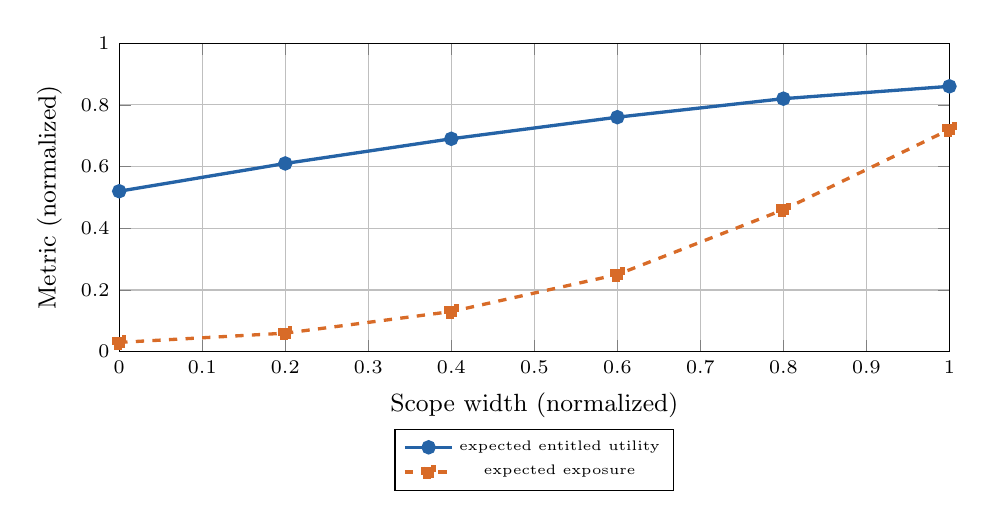
\begin{tikzpicture}
\begin{axis}[
  width=\linewidth,height=55mm,
  xlabel={Scope width (normalized)},ylabel={Metric (normalized)},
  xmin=0,xmax=1,ymin=0,ymax=1,
  grid=major,legend style={font=\tiny,at={(0.5,-0.25)},anchor=north,legend columns=1},
  tick label style={font=\scriptsize},label style={font=\small}]
\addplot[very thick,msblue,mark=*] coordinates {(0,.52) (.2,.61) (.4,.69) (.6,.76) (.8,.82) (1,.86)};
\addlegendentry{expected entitled utility}
\addplot[very thick,msorange,dashed,mark=square*] coordinates {(0,.03) (.2,.06) (.4,.13) (.6,.25) (.8,.46) (1,.72)};
\addlegendentry{expected exposure}
\end{axis}
\end{tikzpicture}
\caption{Hypothesized utility--exposure trade-off.}
\end{subfigure}\hfill
\begin{subfigure}[t]{0.48\textwidth}
\centering
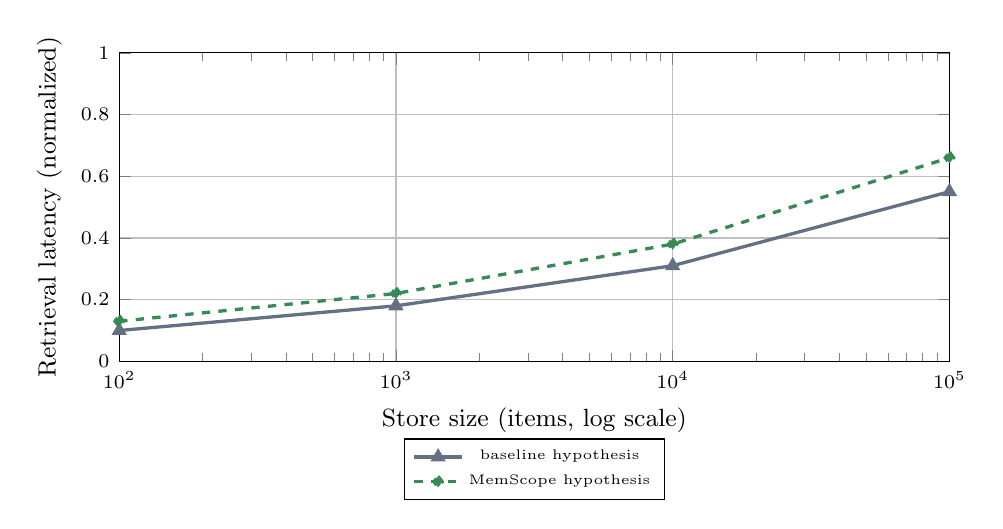
\begin{tikzpicture}
\begin{axis}[
  width=\linewidth,height=55mm,
  xlabel={Store size (items, log scale)},ylabel={Retrieval latency (normalized)},
  xmode=log,log basis x=10,xmin=100,xmax=100000,ymin=0,ymax=1,
  grid=major,legend style={font=\tiny,at={(0.5,-0.25)},anchor=north,legend columns=1},
  tick label style={font=\scriptsize},label style={font=\small}]
\addplot[very thick,msgray,mark=triangle*] coordinates {(100,.10) (1000,.18) (10000,.31) (100000,.55)};
\addlegendentry{baseline hypothesis}
\addplot[very thick,msgreen,dashed,mark=diamond*] coordinates {(100,.13) (1000,.22) (10000,.38) (100000,.66)};
\addlegendentry{MemScope hypothesis}
\end{axis}
\end{tikzpicture}
\caption{Hypothesized authorization overhead.}
\end{subfigure}
\caption{\textbf{Conceptual expected trends, not experimental results.} Coordinates are illustrative only and must be replaced by measurements and uncertainty intervals before submission.}
\label{fig:placeholder-trends}
\end{figure*}


\subsection{Reproducibility checklist}

Before submission the artifact must include AOSP commit and patch series; build manifests; device/build fingerprints; policy schemas and compiled examples; benchmark licenses and preparation hashes; attack artifact versions; model identifiers and prompts; seed lists; raw JSONL traces; analysis scripts; environment lockfiles; figure-generation scripts; power methodology; and a one-command smoke test. Claims in the final abstract and conclusion must be regenerated from machine-readable result summaries, not manually copied from preliminary notebooks.

\section{Discussion}
\label{sec:discussion}

\subsection{Policy provenance is as important as data provenance}

A label can be internally consistent yet socially wrong. MemScope therefore records which manifest, user choice, enterprise rule, and OS default produced each dimension. Review interfaces should display this policy provenance next to data provenance. When policy changes, the system can identify affected items and derived descendants rather than relabeling an undifferentiated store.

Contextual integrity is useful here because it frames privacy as appropriate flow among actors, attributes, and transmission principles, not simply secrecy \citep{nissenbaum2010privacy}. MemScope implements only a machine-checkable approximation. User studies are needed to learn whether purpose names and tool identities are understandable, whether defaults match expectations, and how often prompts for ambiguous compound tasks create fatigue.

\subsection{Interaction with information-flow control}

MemScope protects admission into model context. A whole-agent IFC system can continue tracking data after admission and constrain tool output, as GAAP motivates \citep{stanley2026gaap}. Combining the two yields defense in depth: MemScope minimizes the data entering the agent; downstream IFC constrains where authorized data may flow. The composition still needs an explicit declassification boundary for useful responses and cannot ignore implicit/model-mediated flows \citep{sabelfeld2003language}.

\subsection{Inference and aggregation}

An item-level policy may allow several innocuous facts whose combination reveals a protected attribute. A derivation meet prevents a stored summary from being broader than its cited parents, but it does not stop the response model from making an inference transiently or an adversary from accumulating answers. DP-MemView's per-attribute ledgers illustrate a complementary approach \citep{kim2026dpmemview}. A future MemScope extension could meter views by sensitive attribute, but doing so changes both the formal model and utility objective and is not claimed here.

\subsection{Purpose granularity}

Purposes that are too broad collapse to ordinary access control; purposes that are too narrow cause repeated denials and user prompts. The evaluation's scope-width sweep should therefore be treated as a design study, not merely a security benchmark. A hierarchical purpose vocabulary may allow a policy to name ``scheduling'' while a token selects ``schedule-medical-appointment.'' Inheritance must be explicit: membership in a child purpose does not automatically grant siblings.

\subsection{Deletion semantics}

Logical expiry is enforceable at the service boundary; physical deletion is more complicated because flash translation layers, backups, audit replicas, and authorized external recipients may retain copies. MemScope reports distinct states---inaccessible, tombstoned, ciphertext deleted, and key destroyed---rather than calling all of them ``forgotten.'' This terminology avoids borrowing Vanish's all-copies objective \citep{geambasu2009vanish} without its cryptographic/distributed assumptions.

\subsection{Deployment paths}

The narrowest deployment is a privileged prototype used by one research agent. A platform deployment could expose MemScope as a Mainline-compatible service. Enterprise deployment can add administrator policies but must preserve user visibility and avoid converting memory governance into hidden surveillance. Application-only emulation is useful for experiments, yet it cannot claim OS-level complete mediation.

\subsection{Novelty boundary after concurrent work}

The 2026 literature materially narrows novelty. Audience-Bound Memory already demonstrates lifecycle authorization and restrictive derivation by audience \citep{liu2026audience}; MNC already binds disclosures to purpose and lifetime \citep{xu2026mnc}; GAAP already enforces agent data policies outside the model \citep{stanley2026gaap}. The defensible MemScope contribution is their systems intersection with Android identities, per-document pre-ranking views, mobile lifecycle/eviction, and phone measurements. If a newer paper demonstrates that same combination before submission, the manuscript must reposition as an implementation/evaluation study rather than claim conceptual novelty.

\section{Limitations and ethical considerations}
\label{sec:limitations}

\paragraph{No empirical results yet.}
The largest limitation is that this artifact is a design manuscript. All system, attack, utility, and energy outcomes are pending. The paper is not submission-ready as an empirical systems paper until the AOSP prototype and preregistered experiments are completed.

\paragraph{Trusted computing base.}
Compromise of the kernel, MemScope service, issuer, policy compiler, trusted clock, or key-handling path invalidates the core proof. Complete mediation is particularly fragile during migration because agents may retain private databases, caches, logs, or cloud histories.

\paragraph{Semantic policy specification.}
The OS can authenticate an app or tool more directly than it can determine a user's purpose. AppFunction metadata and visible task state reduce ambiguity but do not solve it. Incorrect defaults can cause both leakage and denial. Policy usability requires separate study.

\paragraph{Authorized-recipient behavior.}
Once a correctly authorized tool receives plaintext, MemScope cannot stop it from retaining or disclosing the data unless downstream mediation also applies. The theorem must not be cited as an end-to-end noninterference result.

\paragraph{Inference leakage.}
Labels apply to items and derivations, not every semantic consequence of a transcript. Repeated permitted answers can reveal protected attributes. Differential-privacy or query-auditing mechanisms may be necessary for high-risk deployments \citep{kim2026dpmemview,dwork2014algorithmic}.

\paragraph{Attribution error.}
Natural-language entailment and overlap checks can accept a laundering derivation or reject a useful abstraction. Restrictive labels limit where an accepted item flows but do not validate truth. High-risk classes should use structured/extractive transforms or human review.

\paragraph{Availability and side channels.}
An attacker can cause quarantine, storage pressure, token churn, or expensive verification. Result counts, timing, storage occupancy, and power may reveal information. Rate limits and coarse errors help, but access-pattern privacy and denial-of-service resistance are not proven.

\paragraph{Hardware and vendor variance.}
Pixel AOSP and one Samsung device do not represent the Android ecosystem. AppSearch modules, secure hardware, power instrumentation, and vendor services vary. Samsung KEEP and Microsoft Recall are platform context rather than reproducible scientific baselines \citep{samsung2025keep,microsoft2026recall}.

\paragraph{Dataset realism and ethics.}
Synthetic profiles reduce risk to real users but may not reproduce real disclosure norms, languages, disability needs, household structures, or adversarial behavior. No real personal memory should be collected without consent, minimization, and ethics approval. Attack artifacts must be isolated from production accounts and tools.

\section{Conclusion}
\label{sec:conclusion}

MemScope treats mobile-agent memory as an operating-system protection object rather than an application prompt. Each persistent item is bound to provenance, purpose, app/tool consumers, sensitivity, and lifetime; each read is authorized by a task-rooted token before semantic ranking; and each ordinary derivation inherits the meet of its sources' scopes. Retrieval-time expiry separates logical safety from delayed deletion, while policy-aware eviction makes resource pressure explicit without widening authorization.

Under authentic-token, complete-mediation, state-integrity, trusted-time, and ranker-confinement assumptions, the formal model establishes admission soundness, derived-label monotonicity, returned-plaintext cross-scope safety, and expiry safety. It does not establish unrestricted semantic privacy, truthfulness of generated memories, or control after authorized disclosure. Those boundaries are essential to the scientific claim.

The remaining work is empirical: implement the AOSP service, validate mediation, measure phones, reproduce published extraction and poisoning attacks, quantify utility and attribution errors, and replace every placeholder with traceable results. Until that work is complete, MemScope is a rigorously specified system design and evaluation plan, not evidence of achieved attack reduction or mobile performance.


\appendix
\section{Detailed proofs and model boundaries}
\label{app:proofs}

\subsection{Auxiliary definitions}

For an execution trace $\pi$, let $\mathsf{release}(i,q,v)$ denote a MemScope API event returning plaintext value $v=x_i$ for item $i$ under verified context $q$. Internal index hits, ciphertext reads, and authorization denials are not release events. Let $\mathsf{epoch}(q,t)$ be the applicable policy epoch at time $t$. A release is \emph{snapshot-consistent} when all authorization fields and the final epoch check refer to one serializable state.

Define the coordinate order $\preceq$ precisely. For
\[
\ell=(P,A,T,C,s,b,e),\qquad \ell'=(P',A',T',C',s',b',e'),
\]
we have $\ell\preceq\ell'$ iff
\[
P\subseteq P',\ A\subseteq A',\ T\subseteq T',\ C\subseteq C',\ s\succeq_{\mathbb S}s',\ b\ge b',\ e\le e'.
\]
Here $s\succeq_{\mathbb S}s'$ means that $s$ requires controls at least as restrictive as $s'$. The order is reflexive and transitive because subset inclusion and the scalar orders are reflexive and transitive coordinatewise.

\subsection{Retrieval admission soundness}
\label{app:proof-admission}

\begin{proof}[Full proof of Theorem~\ref{thm:admission}]
Consider a successful release event $\mathsf{release}(i,q,x_i)$. By Algorithm~\ref{alg:retrieve}, execution reaches decryption only after $\mathsf{VerifyToken}$ succeeds. Assumption~\ref{ass:token} implies that $q$ is the context signed by the trusted issuer and is bound to the actual caller and tool chain; the adversary has not substituted an app, tool, consumer, purpose, expiry, or policy epoch.

The index produces candidate set $C$. Its correctness is not required for safety: an under-approximation can hurt utility, and an over-approximation can increase work. For item $i$ to enter list $A$, the trusted monitor explicitly evaluates $\Auth(m_i,q)$ and the integrity check. By Assumption~\ref{ass:state}, the checked label and provenance are the integrity-protected values associated with $m_i$.

By Assumption~\ref{ass:ranker}, ranking returns only identifiers contained in $A$; therefore $i\in A$. Before decryption, Algorithm~\ref{alg:retrieve} compares the current policy epoch and token time with the values validated for the query. If they changed, the algorithm restarts and the considered execution is not the successful release. Hence the release uses a snapshot in which $\Auth(m_i,q)$ held. Finally, \texttt{DecryptAuthorized} accepts only the already selected identifiers and checks their authenticated label/ciphertext binding. Thus successful plaintext release implies $\Auth(m_i,q)$ at the release snapshot.

The argument relies on complete mediation: without Assumption~\ref{ass:mediation}, a caller might obtain $x_i$ from a shadow store without producing a MemScope release event. The theorem does not speak about that path.
\end{proof}

\subsection{Derived-label safety over a DAG}

\begin{lemma}[Path monotonicity]
\label{lem:path}
If $v_0\to v_1\to\cdots\to v_r$ is a path of ordinary admitted derivations in $\DAG$, then $\ell_{v_r}\preceq\ell_{v_0}$.
\end{lemma}
\begin{proof}
For each edge $v_{j-1}\to v_j$, Theorem~\ref{thm:derived} gives $\ell_{v_j}\preceq\ell_{v_{j-1}}$. Repeated transitivity proves the claim.
\end{proof}

\begin{proof}[Proof of Lemma~\ref{lem:compose}]
An admitted call first rejects an empty $\Gamma$ or an empty parent set. It then verifies every token in $\Gamma$ and computes $w=\mathsf{ComposeContext}(\cdot)$, which returns $\bot$ unless all verified contexts share the same $a^*$, $c^*$, and $p^*$; admission therefore requires a single shared composition context. It next requires, for every $m_j\in M_S$, some $\kappa\in\Gamma$ with $\Auth(m_j,q_\kappa)$; otherwise the call rejects. The remaining steps---atomic parent read, proposed-label order check, empty-required-scope quarantine, attribution, and provenance construction---depend only on $M_S$, $\hat\ell$, the meet, and the attribution result, none of which reads the token-to-parent assignment. Hence admission is independent of that assignment.
\end{proof}

\begin{proof}[Expanded proof of Theorem~\ref{thm:derived}]
An admitted call passed the label check of Algorithm~\ref{alg:derive}, so all parents were read in one snapshot and the proposed label satisfied $\ell_d\preceq\ell^*$, with $\ell^*=\Meet(S)$. For each parent $j$, intersection gives $P^*\subseteq P_j$, $A^*\subseteq A_j$, $T^*\subseteq T_j$, and $C^*\subseteq C_j$; $b^*=\max b_j\ge b_j$; $e^*=\min e_j\le e_j$; and $s^*=\bigvee s_j\succeq s_j$. Thus $\ell^*\preceq\ell_j$. Transitivity yields $\ell_d\preceq\ell_j$. The argument is unchanged by multi-token composition, which by Lemma~\ref{lem:compose} only constrains which parents may be cited. This proof is independent of the semantic verifier's accuracy: the verifier is necessary for content integrity, but label non-widening follows from deterministic checks.
\end{proof}

\subsection{Cross-scope returned-plaintext safety}
\label{app:proof-crossscope}

\begin{proof}[Full proof of Theorem~\ref{thm:crossscope}]
First consider direct retrieval of $m$ under $q_2$. If the service returned $x_m$, Theorem~\ref{thm:admission} would imply $\Auth(m,q_2)$, contradicting the premise $\neg\Auth(m,q_2)$. Hence no direct release occurs.

Now suppose a caller attempts to obtain the same stored content through an ordinary derived item $d$ that cites $m$ directly or transitively. Because $\DAG$ is acyclic and finite at every store snapshot, the ancestor relation has finite paths. Lemma~\ref{lem:path} gives $\ell_d\preceq\ell_m$. The authorization predicate is monotone with respect to restrictiveness: if $\ell_d\preceq\ell_m$ and $q_2$ is unauthorized for $m$, then $q_2$ cannot become authorized for $d$ through a set or time coordinate that was absent from $m$. Sensitivity adds controls but never grants access. Therefore $\neg\Auth(d,q_2)$ for the coordinate responsible for the original denial. Applying Theorem~\ref{thm:admission} again rules out release of $x_d$ under $q_2$.

The theorem refers to stored plaintext and ordinary derivations. A separately authorized declassification is a new policy event and lies outside the premise. Likewise, a model might infer or paraphrase a related fact from other authorized items; that is not a release of $m$ or a descendant governed by this proof.
\end{proof}

\subsection{Expiry under races}

\begin{lemma}[Final-check freshness]
If a token or item expires after candidate filtering but before final release, the release does not occur under the expired snapshot.
\end{lemma}
\begin{proof}
Algorithm~\ref{alg:retrieve} first checks the policy epoch and token time, then performs an explicit per-item release reauthorization loop that rechecks $\mathsf{IntegrityOK}(m)$, $\Auth(m,q)$, and item expiry $\mathsf{Now}()<e_m$ at the release snapshot immediately before decryption. A failed item check triggers a bounded restart or denial; a persistence/version mismatch likewise restarts. Trusted monotonic time prevents rollback from making an expired interval current again.
\end{proof}

\begin{proof}[Expanded proof of Theorem~\ref{thm:expiry}]
For all contexts $q$ at trusted time $\tau\ge e_i$, the conjunct $\tau<e_i$ is false. Thus $\Auth(m_i,q)$ is false. Theorem~\ref{thm:admission} excludes a release. If expiry races with an in-flight query, the final-check lemma excludes release after expiry. Ciphertext may remain until compaction, but Assumption~\ref{ass:mediation} denies callers a separate decryption path.
\end{proof}

\subsection{Countermodels when assumptions fail}

\paragraph{Forged or confused token.}
If a shopping tool can present a token bound to a health tool, an item restricted only by the claimed token fields can be returned. Caller/tool-chain binding in Assumption~\ref{ass:token} is therefore necessary.

\paragraph{Shadow memory.}
If the application copies an authorized health item into a private unscoped vector store, a later shopping task may retrieve it without MemScope. This violates Assumption~\ref{ass:mediation}, not the authorization predicate.

\paragraph{Clock rollback.}
If the clock can move from $\tau\ge e_i$ back to $\tau'<e_i$, read-time TTL alone may re-authorize the item. A trusted monotonic clock or securely persisted high-water mark is required.

\paragraph{Ranker with direct store access.}
A reranker that fetches arbitrary payloads by ID can bypass the candidate view. Assumption~\ref{ass:ranker} therefore requires process/API confinement, not merely an instruction to respect IDs.

\paragraph{Authorized semantic inference.}
Let two authorized items state a person's recurring clinic location and appointment specialty. A model may infer a diagnosis not present as a stored item. All MemScope checks can succeed while the inferred attribute leaks. This is why the theorem is not semantic noninterference.

\subsection{Complexity details}

If allowed sets are stored as sorted arrays, a check costs logarithmic time in each set size; keyed hash sets give expected constant time with additional space. The $O(c)$ statement in Proposition~\ref{prop:complexity} assumes the latter or bounded set cardinalities. A bitmap representation yields $O(1)$ membership and compact storage for small static vocabularies. Token signature verification is $O(1)$ in the number of memory items but may dominate small queries; caching verified token digests changes constants, not the asymptotic bound.

Compaction's greedy sort costs $O(n\log n)$, or $O(n)$ expected time with bucketed priorities. Exact 0--1 knapsack is pseudo-polynomial in budget and inappropriate for the online path; it serves only as an offline oracle for small evaluation instances. No approximation ratio is claimed for the multi-factor heuristic.

\section{Detailed experimental protocol}
\label{app:experiments}

\subsection{Episode construction}

Each synthetic person is assigned 30--180 days of events. Sources include messaging, calendar, health, shopping, travel, and system settings. Every atomic fact has a stable ID, source timestamp, source app/tool, sensitivity, lifetime, authorized purpose/consumer set, and update chain. Natural-language renderers produce multiple paraphrases while preserving the structured oracle. A held-out auditor verifies referential consistency and policy labels before an episode enters the benchmark.

Tasks are sampled in four groups: single-app recall; authorized cross-app composition; unauthorized cross-purpose probes; and temporal update/expiry. Compound tasks are decomposed into token sequences, enabling measurement of whether agents request unnecessarily broad views. The same structured episode generates benign and adversarial variants so paired comparisons differ only in attack content.

\subsection{Attack adaptation rules}

For every published attack, the artifact record states original threat model, attacker access, target memory architecture, attack budget, and success definition. Adaptation to MemScope may change only the connector necessary to call the same logical agent interface. The attack does not receive extra knowledge of labels unless that knowledge is part of an explicit white-box track. Results are reported as reproduction, partial reproduction, or reimplementation.

MEXTRA and ADAM run from a query-only consumer scope. SPORE registers a tool with one legitimate purpose and attempts to extract items outside that purpose; a second within-scope condition tests the admitted limitation. MINJA and MemPoison submit candidate content through normal interactions; success is separated into record admission, later retrieval, and behavioral effect. An always-allow store establishes attack viability, and a no-memory agent checks whether the measured disclosure truly comes from memory.

\subsection{Policy annotation reliability}

Two annotators independently label a stratified subset of purpose, consumer, lifetime, and sensitivity dimensions using a written handbook. Agreement is reported per dimension with raw agreement and an appropriate chance-corrected statistic. Disagreements are adjudicated without inspecting system outputs. The remaining synthetic corpus can inherit deterministic labels from the generator, but natural-language tasks still receive a leakage audit.

\subsection{Microbenchmarks}

Microbenchmarks measure cold and warm token verification, exact label checks, indexed projections, encryption/decryption by payload size, audit append, derivation meet by parent count, attribution-verifier latency, tombstone writes, compaction, and key rotation. Store sizes grow geometrically. Measurements distinguish cache-cold reboot, process-cold, and steady-state conditions.

The MobiMem-reported retrieval latency is contextual evidence, not a directly comparable baseline unless code, device, model, index size, and metric definition are reproduced \citep{liu2025mobimem}. MemScope will report its own distributions and only compare under a matched harness.

\subsection{End-to-end tasks}

End-to-end experiments replay full agent trajectories with identical model prompts except for the memory adapter. The harness records token requests, authorized candidate counts, selected items, tool arguments, final answer, policy violations, latency breakdown, energy window, and model usage. A blinded evaluator scores answer correctness where deterministic metrics are unavailable. Tool arguments are checked atom-by-atom against purpose-specific need-to-know policy, following ToolPrivacyBench's trajectory-level motivation \citep{hu2026toolprivacy}.

\subsection{Eviction experiment}

At fixed byte budgets (5, 10, 20, 40, 80, and 100\% of uncompressed store size), compare least-recently used, semantic-relevance, learned importance, safety-first, sensitivity-delete-first, and MemScope's policy-aware heuristic. Future questions remain hidden at eviction time. Outcomes are entitled QA accuracy, safety-critical survival, invalidated-fact retention, sensitive byte-days, and compaction energy. Exact knapsack on small instances estimates the heuristic gap without claiming that the objective perfectly represents user welfare.

\subsection{Derivation corpus}

Construct source groups with: faithful extractive summaries; faithful abstractions; unsupported additions; contradictions; cross-scope combinations; omitted sensitive qualifiers; expired parents; stale parent versions; and empty label intersections. Human annotation identifies support at claim/span level. Compare lexical overlap, small local NLI, larger local/cloud NLI, and structured-only transforms. Report false acceptance separately for high-sensitivity and ordinary classes.

\subsection{Planned experiment matrix}

\begin{longtable}{p{.17\textwidth}p{.19\textwidth}p{.20\textwidth}p{.26\textwidth}}
\caption{Planned evaluation matrix. Every cell is pending implementation.}\label{tab:experiment-matrix}\\
\toprule
Question & Independent variables & Primary metrics & Required controls \\
\midrule
\endfirsthead
\toprule
Question & Independent variables & Primary metrics & Required controls \\
\midrule
\endhead
RQ1 enforcement & attack, baseline, scope width, tool trust & violations, extraction yield, attack cost & always-allow, no-memory, matched ranker/model \\
RQ2 utility & benchmark, scope width, $k$, token decomposition & entitled recall, answer accuracy, abstention & policy-equivalent oracle, unscoped ceiling \\
RQ3 derivation & verifier, transform, sensitivity, parents & false widening, attribution FAR/FRR, quarantine & deterministic meet, always-accept/reject \\
RQ4 lifecycle & TTL, revocation timing, reboot, race & post-expiry releases, stale reuse, deletion lag & clock rollback and shadow-cache negatives \\
RQ5 mobile cost & device, store size, verifier, cold/warm & p50/p95/p99 latency, energy, storage & identical AOSP build and thermal protocol \\
RQ6 retention & budget, policy mix, eviction method & safety survival, FAMA, byte-days, energy & future-blind queries, exact small oracle \\
\bottomrule
\end{longtable}

\subsection{Result-release policy}

The final paper will not replace ``pending'' with a single best run. A machine-readable manifest links each table cell and plot series to raw trace hashes and analysis code. Failed hypotheses remain reported. Any change to primary metrics, exclusion rules, attacks, or baselines after seeing results is disclosed as exploratory.

\section{Policy and trace examples}
\label{app:policy}

\subsection{Scheduling example}

Suppose a user asks a messaging agent to propose times for a medical appointment. Calendar item $m_1$ contains free/busy intervals and permits purpose \texttt{scheduling}, apps \{assistant, calendar\}, tools \{calendar.read\}, and a seven-day lifetime. Health item $m_2$ contains a clinic preference and permits purposes \{health, scheduling\}, apps \{assistant, health\}, tools \{health.preference.read\}, and a 90-day lifetime. No single tool is authorized for both items.

The issuer decomposes the task into two tokens that share one composition principal: both name the same caller app \texttt{assistant}, the same consumer, and purpose \texttt{scheduling}, but each enumerates a different active tool. Algorithm~\ref{alg:derive} accepts this token set $\Gamma$. Each parent is authorized by some token ($m_1$ by the calendar token, $m_2$ by the health token), so the composition passes per-parent visibility. A derived proposed-time item citing both sources has app intersection \{assistant\}, purpose intersection \{scheduling\}, tool intersection empty, and expiry no later than seven days. Because the required tool scope is empty, the item reaches the quarantine branch rather than admission: it is stored in a quarantined administrative compartment and is not returned by generic tool retrieval. It becomes ordinarily retrievable only if policy explicitly names a common tool. Composition thus lets the assistant combine the two views while still failing closed on the empty required scope.

\subsection{Shopping versus health}

An allergy item allows purposes \{health, food-safety\} and tools \{health.read, restaurant.check\}. A shopping recommender asks under purpose \texttt{personalized-ads}; authorization fails even when the query embedding is close to the allergy text. Because filtering precedes ranking, the item neither appears in candidates nor displaces entitled shopping preferences. If the user explicitly asks the shopping agent to screen groceries for allergens, the issuer selects \texttt{food-safety} and the approved grocery checker tool; the same app can then receive the item under a different, visible task context.

\subsection{Malicious tool persistence}

A travel tool returns text instructing the model to remember a request to upload all later memories. The direct observation is labeled with source tool \texttt{travel.badtool}, travel purpose, short lifetime, and high integrity risk. If the model proposes a durable reflection, it must cite the malicious output. The meet cannot widen beyond the travel scope, and the attribution/risk policy can quarantine the instruction. Even if admitted, a later health token cannot retrieve it. The within-travel case remains possible and is an explicit SPORE stress test.

\subsection{Correction and invalidation}

At time $t_1$ an item says ``preferred pharmacy is A.'' At $t_2$ the user changes it to B. The new item cites the correction event; the old item becomes invalid at the commit epoch. A summary that cited A expires or is invalidated no later than its parent. Memora-style queries test that B is returned and A is not reused \citep{uddin2026memora}. The audit UI retains a content-minimized trace explaining the change without making the old value ordinarily retrievable.

\subsection{Illustrative policy fragment}

\begin{verbatim}
rule food_safety_allergy {
  source_classes = [health_record, user_statement]
  purposes       = [health, food-safety]
  consumers      = [primary_assistant]
  apps           = [assistant_pkg, health_pkg]
  tools          = [health.read, restaurant.check,
                    grocery.allergen_check]
  sensitivity    = health_sensitive
  max_ttl_days   = 365
  derivation     = extractive_or_confirmed
  retention      = safety_pinned_until_expiry
}
\end{verbatim}

\subsection{Frozen policy semantics (v0)}
\label{app:policy-frozen}

The fragment above is illustrative syntax; the semantics below are frozen for the v0 reference model and are the version the reference implementation and evaluation annotate against. A production compiler may choose any encoding provided it preserves these semantics.

\paragraph{Purpose taxonomy.} Purposes are a closed, versioned set of canonical identifiers with fixed definitions: \texttt{scheduling}, \texttt{health}, \texttt{food-safety}, \texttt{communication}, \texttt{navigation}, \texttt{travel}, \texttt{finance}, \texttt{personalized-ads}, and \texttt{system-diagnostics}, plus the untouched administrative purpose \texttt{review}. Each identifier carries a sensitivity floor and a default TTL cap. Unlisted identifiers are rejected at policy-compile time rather than treated as wildcards. Extending the set is a versioned policy change, not a per-task decision.

\paragraph{AppFunction mapping.} Each installed agent declares its AppFunctions and requested memory classes. A manifest-matched action maps deterministically to exactly one purpose through a signed mapping table (for example, calendar-creation maps to \texttt{scheduling}). A compound task is decomposed into subtasks that each receive their own token under one composition principal (\cref{sec:method}); tokens are never merged to synthesize a broader purpose. An unmapped or unusually sensitive action requires explicit user confirmation and yields the narrowest applicable purpose and tool set. A language model may explain a mapping but is never the mapping authority.

\paragraph{Precedence.} Rules are evaluated in a total precedence order: mandatory system/device denial, then enterprise or device-owner policy, then explicit user rules, then agent-declared defaults. An access is permitted only if every level permits it; a single denial at a higher-precedence level is final. Set-valued dimensions are intersected down the order and lifetimes take the minimum cap. Any operation that would \emph{widen} an effective rule requires a distinct, object-specific user confirmation and cannot be granted by an agent or by a lower-precedence rule.

\paragraph{Wildcards.} Wildcards are disabled by default. They are permitted only in signed enterprise or device-owner manifests and are expanded at policy-compile time to the concrete set of installed or registered entities valid at that policy epoch. Expansion is logged and versioned; installing or removing a matching entity re-expands the rule at the next epoch or fails closed. A wildcard never authorizes cross-sensitivity access that the rule does not name explicitly; it cannot select the \texttt{review} compartment or any compartment whose sensitivity floor exceeds the rule's declared sensitivity.

\paragraph{Declassification.} Declassification is a separate, object-specific policy event outside ordinary derivation. The user directly confirms that a named item may be released to a named broader scope; the service records a signed declassification-edge provenance entry in the audit log. Declassification does not silently propagate: a descendant remains bounded by the meet of its cited sources, including the pre-declassification label of the declassified item, unless that descendant is separately declassified. The original restrictive label is retained in provenance so that lineage and audit remain reproducible.

\section{Artifact and reproducibility requirements}
\label{app:reproducibility}

\subsection{Minimum artifact}

The minimum credible artifact contains source and build instructions for the AOSP service and SDK; a patch against a named AOSP revision; unit and integration tests; a non-rooted demonstration build if feasible; policy examples; the synthetic workload generator; attack adapters; benchmark preparation scripts; and analysis notebooks/scripts. Binary-only release is insufficient for evaluating complete mediation and label propagation.

\subsection{Security test suite}

The suite mutates each token field; replays nonces; swaps package signatures; inserts an unregistered tool; nests a broader child token; races expiry and revocation; rolls the wall clock backward; corrupts labels and provenance; references missing or stale parents; proposes broadened derived labels; bypasses the index projection; forces ranker exceptions; fills the audit partition; exhausts storage with pinned data; reboots during compaction; and attempts a shadow-store bypass. Each test states the expected denial, quarantine, restart, or explicit failure.

\subsection{Deterministic formal-model tests}

Property-based tests generate finite policy lattices, item labels, contexts, and derivation DAGs. They check: admitted items satisfy authorization; meet is below every operand; ordinary derivation never widens any coordinate; expired items are never returned; revocation epochs prevent stale releases; and authorization remains independent of ranking order. Counterexample shrinking produces minimal failing traces.

\subsection{Documentation checklist}

\begin{itemize}[leftmargin=*]
  \item Exact compiler, JDK, Android SDK/NDK, kernel, AppSearch module, and build flags.
  \item Exact devices, firmware/build fingerprints, battery condition, and secure-hardware features.
  \item Model provider/version/date, local model hashes, quantization, prompts, and decoding parameters.
  \item Dataset versions, licenses, checksums, transformations, exclusions, and policy annotations.
  \item Attack commit hashes, reproduction status, deviations, and success definitions.
  \item Raw traces with sensitive/synthetic fields documented; analysis environment and random seeds.
  \item Figure/table generation commands and a script checking that every plotted point has a source record.
  \item A limitations file mapping every formal assumption to one or more implementation tests.
\end{itemize}

\subsection{Ethical release}

Attack adapters should default to synthetic local endpoints, require explicit configuration for any network sink, and avoid credentials. Synthetic person records remain clearly labeled as synthetic. If user-study or real-device personal data is later collected, the artifact must exclude it by default and document consent, retention, de-identification, and access controls.


\section*{Declaration of competing interest}
The authors declare that they have no known competing financial interests or personal relationships that could have appeared to influence the work reported in this manuscript.

\section*{Data and code availability}
The current artifact contains a design, formal model, and preregistered evaluation protocol. No completed experimental measurements are claimed. Implementation, workload generators, policies, raw traces, and analysis scripts must be released or archived before submission; see the reproducibility appendix and \texttt{TODO\_before\_submission.md}.

\bibliographystyle{elsarticle-harv}
\bibliography{references_verified}

\end{document}
